\documentclass[12pt]{hcmut-report}

\usepackage{graphicx}
\usepackage{tabularx}
\usepackage{enumitem}
\usepackage{titlesec}
\usepackage{tocloft}
\usepackage{longtable}
\usepackage{array}
\usepackage{pdflscape}
\usepackage{etoolbox}
\usepackage{xurl}

% Định dạng hệ thống đề mục theo mẫu: 1., 2., ... và a., b., ...
% Mục lục chỉ hiển thị hai cấp section/subsection.
\renewcommand{\contentsname}{Mục lục}
\renewcommand{\figurename}{Hình}
\renewcommand{\tablename}{Bảng}
\renewcommand{\listfigurename}{Danh mục hình ảnh}
\renewcommand{\listtablename}{Danh mục bảng}
% babel nạp lại tên tiếng Anh ở đầu tài liệu; khai báo trong captionsenglish
% để các tiêu đề và chú thích luôn giữ đúng tiếng Việt.
\addto\captionsenglish{%
  \renewcommand{\contentsname}{Mục lục}%
  \renewcommand{\figurename}{Hình}%
  \renewcommand{\tablename}{Bảng}%
  \renewcommand{\listfigurename}{Danh mục hình ảnh}%
  \renewcommand{\listtablename}{Danh mục bảng}%
}
\captionsetup{%
  font=small,
  labelfont=bf,
  labelsep=period,
  justification=centering,
  singlelinecheck=true,
  skip=6pt
}
\renewcommand{\thesubsection}{\alph{subsection}}
\setcounter{tocdepth}{2}
\renewcommand{\cftsecaftersnum}{.}
\renewcommand{\cftsubsecaftersnum}{.}
\renewcommand{\cftsecleader}{\hfill}
\AtBeginDocument{%
  \counterwithout{equation}{section}%
  \counterwithout{table}{section}%
  \counterwithout{figure}{section}%
}

\makeatletter
\patchcmd{\LT@output}{\copy\LT@foot\vss}{\copy\LT@foot\vfil}{}{}
\patchcmd{\LT@output}{\copy\LT@foot\vss}{\copy\LT@foot\vfil}{}{}
\makeatother

\usepackage{natbib}
\setcitestyle{numbers,square}

\titleformat{\section}
  {\normalfont\bfseries\fontsize{14}{17}\selectfont}
  {\thesection.}{0.5em}{}
\titleformat{\subsection}
  {\normalfont\bfseries\fontsize{13}{16}\selectfont}
  {\thesubsection.}{0.5em}{}
\titleformat{\subsubsection}
  {\normalfont\bfseries\normalsize}
  {\thesubsubsection.}{0.5em}{}

\titlespacing*{\section}{0pt}{1.5ex plus 0.5ex}{0.8ex}
\titlespacing*{\subsection}{0pt}{1.2ex plus 0.4ex}{0.6ex}
\titlespacing*{\subsubsection}{0pt}{1ex plus 0.3ex}{0.4ex}

\newenvironment{nfrdetails}{%
  \begin{itemize}[
    label=\textbullet,
    leftmargin=1.6em,
    itemsep=5pt,
    parsep=0pt,
    topsep=5pt
  ]
}{\end{itemize}}

\newenvironment{reportitems}{%
  \begin{itemize}[
    label=\textbullet,
    leftmargin=1.6em,
    itemsep=4pt,
    parsep=0pt,
    topsep=4pt
  ]
}{\end{itemize}}

\newcolumntype{C}[1]{>{\centering\arraybackslash}p{#1}}
\newcolumntype{U}[1]{>{\bfseries\raggedright\arraybackslash}p{#1}}

\definecolor{ucRule}{RGB}{150,174,195}

\setlength{\parindent}{0pt}
\setlength{\headheight}{37pt}
\raggedbottom
\hbadness=10000
\vbadness=10000
\newcommand{\firstparagraph}{\noindent\hspace*{2em}}

\deptname{Khoa Khoa học và Kỹ thuật Máy tính}
\coursename{HỌC MÁY -- CO3117}
\reporttype{BÁO CÁO BÀI TẬP LỚN}
\title{%
  \parbox{\linewidth}{\centering
    PHÂN LOẠI CHỦ ĐỀ TIN TỨC\par
    TRÊN BỘ DỮ LIỆU AG NEWS\par
  }%
}
\author{}
\advisor{VÕ THANH HÙNG}
\studygroup{20 -- Lớp L03}
\reportplace{Thành phố Hồ Chí Minh}
\reporttime{Tháng 11 năm \the\year}
\stuname{%
  \begin{tabular}{rl}
    1. & Nguyễn Mai Việt Hòa -- 2411141 \\
    2. & Ngô Tuấn Khôi -- 2411697 \\
    3. & Nguyễn Đăng Gia Đạo -- 2410652
  \end{tabular}%
}

\begin{document}

\coverpage

\clearpage
\tableofcontents

\clearpage
\addcontentsline{toc}{section}{Danh mục hình ảnh}
\listoffigures

\clearpage
\addcontentsline{toc}{section}{Danh mục bảng}
\listoftables

\clearpage

\section*{Tóm tắt}
\addcontentsline{toc}{section}{Tóm tắt}

\firstparagraph Báo cáo trình bày quy trình xây dựng và đánh giá một pipeline học máy có giám sát nhằm phân loại bản tin ngắn thành bốn chủ đề: Thế giới (World), Thể thao (Sports), Kinh doanh (Business) và Khoa học/Công nghệ (Sci/Tech) trên bộ dữ liệu AG News. Bộ dữ liệu cân bằng gồm \textbf{120.000} mẫu huấn luyện và \textbf{7.600} mẫu kiểm tra. Nhóm chia tiếp tập huấn luyện thành 85\% train và 15\% validation (\textbf{102.000}/\textbf{18.000} mẫu) để so sánh mô hình trước khi đánh giá lần cuối trên tập test. Nhóm áp dụng quy trình xử lý ngôn ngữ tự nhiên (NLP) để làm sạch văn bản, xóa URL, tách từ, loại bỏ stopword và chuẩn hóa từ. Sau đó, nhóm trích xuất đặc trưng bằng Bag-of-Words (BoW) và TF--IDF với không gian vector tối đa \textbf{5.000} từ.

Để đánh giá hiệu năng, nhóm huấn luyện sáu tổ hợp mô hình dựa trên ba thuật toán truyền thống: Multinomial Naive Bayes, Logistic Regression và Linear SVM.

Kết quả trên tập validation cho thấy mọi mô hình đều vượt xa đường cơ sở dự đoán ngẫu nhiên. Tổ hợp Linear SVM kết hợp TF--IDF đạt hiệu năng cao nhất, với độ chính xác (accuracy) \textbf{0,9138} và macro-F1 \textbf{0,9136}. Thời gian huấn luyện của cấu hình này khoảng \textbf{2,79 giây}. Trên tập test độc lập, cùng cấu hình này đạt accuracy \textbf{0,9051} và macro-F1 \textbf{0,9049}.

Phân tích lỗi cho thấy chủ đề Thể thao có độ phân biệt rõ nhất, trong khi phần lớn lỗi phân loại xuất phát từ sự chồng lấn từ vựng giữa Kinh doanh và Khoa học/Công nghệ. Thử nghiệm bổ sung về lựa chọn đặc trưng bằng kiểm định Chi-bình phương ($\chi^2$) cho thấy việc giữ trọn vẹn 5.000 từ vựng mang lại độ chính xác cao nhất ($0{,}9138$), hạn chế việc đánh mất các từ vựng đặc trưng theo từng chủ đề.

\clearpage
\section*{Phân công công việc}
\addcontentsline{toc}{section}{Phân công công việc}

\firstparagraph Nhóm phân công công việc cụ thể và cân bằng giữa ba thành viên, đảm bảo mỗi thành viên đều tham gia đầy đủ cả phần nghiên cứu lý thuyết, biên soạn báo cáo học thuật và trực tiếp lập trình, kiểm thử các module mã nguồn machine learning của dự án. Tỷ lệ hoàn thành công việc của từng thành viên đạt 100\% theo đánh giá và xác nhận chung của toàn nhóm.

\begin{table}[H]
  \centering
  \caption{Phân công chi tiết nội dung báo cáo và mã nguồn lập trình}
  \label{tab:contribution}
  \footnotesize
  \renewcommand{\arraystretch}{1.35}
  \setlength{\tabcolsep}{4pt}
  \begin{tabularx}{\textwidth}{|>{\raggedright\arraybackslash}p{2.6cm}|C{1.5cm}|>{\raggedright\arraybackslash}p{3.8cm}|>{\raggedright\arraybackslash}X|C{1.3cm}|}
    \hline
    \textbf{Họ tên} & \textbf{MSSV} & \textbf{Nội dung báo cáo} & \textbf{Module mã nguồn đảm nhiệm} & \textbf{Tiến độ} \\
    \hline
    Nguyễn Mai Việt Hòa \par\textit{(Nhóm trưởng)} & 2411141 & Tổng quan bài toán, Nguồn dữ liệu \& Phân tích khám phá (EDA); Đánh giá kiểm thử tập Test; Tổ chức mã nguồn & 
    \textbullet\ \texttt{src/data\_loader.py}\par
    \textbullet\ \texttt{notebooks/}\allowbreak\texttt{01\_data\_}\allowbreak\texttt{analysis.ipynb}\par
    \textbullet\ \texttt{notebooks/}\allowbreak\texttt{04\_final\_}\allowbreak\texttt{test\_evaluation.ipynb}\par
    \textbullet\ \texttt{Dockerfile}, \texttt{requirements.txt}, \texttt{README.md} & 100\% \\
    \hline
    Ngô Tuấn Khôi & 2411697 & Chuẩn bị dữ liệu \& Tiền xử lý; Biểu diễn đặc trưng (BoW, TF--IDF); Thí nghiệm Lựa chọn đặc trưng (Feature Selection); Kết luận \& Hướng phát triển & 
    \textbullet\ \texttt{src/preprocessing.py}\par
    \textbullet\ \texttt{src/utils.py}\par
    \textbullet\ \texttt{notebooks/}\allowbreak\texttt{02\_preprocessing.ipynb}\par
    \textbullet\ \texttt{experiments/}\allowbreak\texttt{feature\_selection.py} ($\chi^2$, Mutual Info, Tree-based) & 100\% \\
    \hline
    Nguyễn Đăng Gia Đạo & 2410652 & Cơ sở toán học các mô hình ML; Thiết kế thực nghiệm \& Huấn luyện (Validation); Thảo luận \& Phân tích lỗi & 
    \textbullet\ \texttt{src/models/baseline.py}\par
    \textbullet\ \texttt{src/models/}\allowbreak\texttt{traditional\_ml.py}\par
    \textbullet\ \texttt{src/evaluation.py}\par
    \textbullet\ \texttt{notebooks/}\allowbreak\texttt{03\_model\_training.ipynb} & 100\% \\
    \hline
  \end{tabularx}
\end{table}

\clearpage
\section{Tổng quan bài toán và dữ liệu}

\firstparagraph Bài toán của báo cáo là phân loại văn bản có giám sát. Với mỗi bản tin, mô hình dự đoán một trong bốn chủ đề. Nhóm sử dụng AG News -- bộ dữ liệu gồm các bản tin ngắn đã có nhãn cùng phép chia sẵn tập huấn luyện và tập kiểm tra. Đặc điểm dữ liệu đặt ra hai yêu cầu khi đánh giá: nhóm cần xử lý các biến thể và nhiễu trong văn bản, đồng thời phải xem xét sự chồng lấn từ vựng giữa một số chủ đề. Ngoài ra, các biểu diễn túi từ được dùng trong báo cáo không mã hóa thứ tự từ, nên chúng không giữ lại toàn bộ ngữ cảnh của câu.

AG News gồm bốn chủ đề: World (Thế giới), Sports (Thể thao), Business (Kinh doanh) và Sci/Tech (Khoa học/Công nghệ). Nhóm giữ nguyên phép chia chính thức gồm 120.000 mẫu huấn luyện và 7.600 mẫu kiểm tra (khoảng 94\% và 6\% tổng số mẫu). Để chọn mô hình và tránh tối ưu trực tiếp trên tập test, nhóm chia thêm tập huấn luyện thành 85\% train và 15\% validation bằng \texttt{train\_test\_split} với \texttt{stratify} và \texttt{random\_state=42}, tương ứng 102.000 và 18.000 mẫu. Mỗi bản ghi có ba trường: \texttt{class} (nhãn từ 1 đến 4), \texttt{title} (tiêu đề) và \texttt{description} (mô tả). Hai trường văn bản được dùng làm nội dung đầu vào ở các bước tiếp theo.

\noindent\textbf{Ví dụ bản ghi.} Bảng dưới đây minh họa hai mẫu dữ liệu theo các trường \texttt{class}, \texttt{title} và \texttt{description}.

\begingroup
\small
\renewcommand{\arraystretch}{1.35}
\setlength{\tabcolsep}{8pt}
\noindent\begin{tabularx}{\textwidth}{>{\centering\arraybackslash}p{1cm}>{\raggedright\arraybackslash}p{4.2cm}>{\raggedright\arraybackslash}X}
  \toprule
  \textbf{class} & \textbf{title} & \textbf{description} \\
  \midrule
  1 & Millions Wait Hours in Venezuela to Vote in Recall Election & The unprecedented vote was sluggish as huge crowds lined up at voting booths. Results were not expected until 8 p.m., or later. \\
  \addlinespace[5pt]
  2 & Leonard Forges Two Clear with Nine to Play at PGA & KOHLER, Wisconsin (Reuters) - American Justin Leonard stayed on track for his second major title in the U.S. PGA Championship final round on Sunday, moving two shots clear with nine holes to play. \\
  \bottomrule
\end{tabularx}
\endgroup

\subsection{Nguồn dữ liệu}

\firstparagraph Nhóm lấy dữ liệu từ trang \textit{AG News Classification Dataset} trên nền tảng Kaggle. Thông tin nhận diện nguồn và thời điểm truy cập được liệt kê dưới đây.

\begin{reportitems}
  \item \textbf{Nền tảng cung cấp:} Kaggle.
  \item \textbf{Tên bộ dữ liệu:} AG News Classification Dataset.
  \item \textbf{Đường dẫn truy cập:} \url{https://www.kaggle.com/datasets/amananandrai/ag-news-classification-dataset}.
  \item \textbf{Ngày truy cập:} 21/09/2026.
\end{reportitems}

Phân phối nhãn trong hai tập dữ liệu được trình bày ở Bảng~\ref{tab:label-distribution}. Các lớp có cùng số lượng mẫu trong từng tập.

\begin{table}[H]
  \centering
  \caption{Phân phối nhãn trên hai tập dữ liệu}
  \label{tab:label-distribution}
  \small
  \renewcommand{\arraystretch}{1.15}
  \setlength{\tabcolsep}{12pt}
  \begin{tabular}{clrrr}
    \toprule
    \textbf{Nhãn} & \textbf{Chủ đề} & \textbf{Huấn luyện} & \textbf{Kiểm tra} & \textbf{Tỉ lệ mỗi tập} \\
    \midrule
    1 & World    & 30.000 & 1.900 & 25\% \\
    2 & Sports   & 30.000 & 1.900 & 25\% \\
    3 & Business & 30.000 & 1.900 & 25\% \\
    4 & Sci/Tech & 30.000 & 1.900 & 25\% \\
    \midrule
    \multicolumn{2}{l}{\textbf{Tổng}} & \textbf{120.000} & \textbf{7.600} & \textbf{100\%} \\
    \bottomrule
  \end{tabular}
  \par\vspace{3pt}
  \parbox{0.86\textwidth}{\footnotesize\textit{Ghi chú:} Tỉ lệ được tính riêng trên từng tập dữ liệu. Mỗi lớp chiếm đúng một phần tư số mẫu.}
\end{table}

\begin{figure}[H]
  \centering
  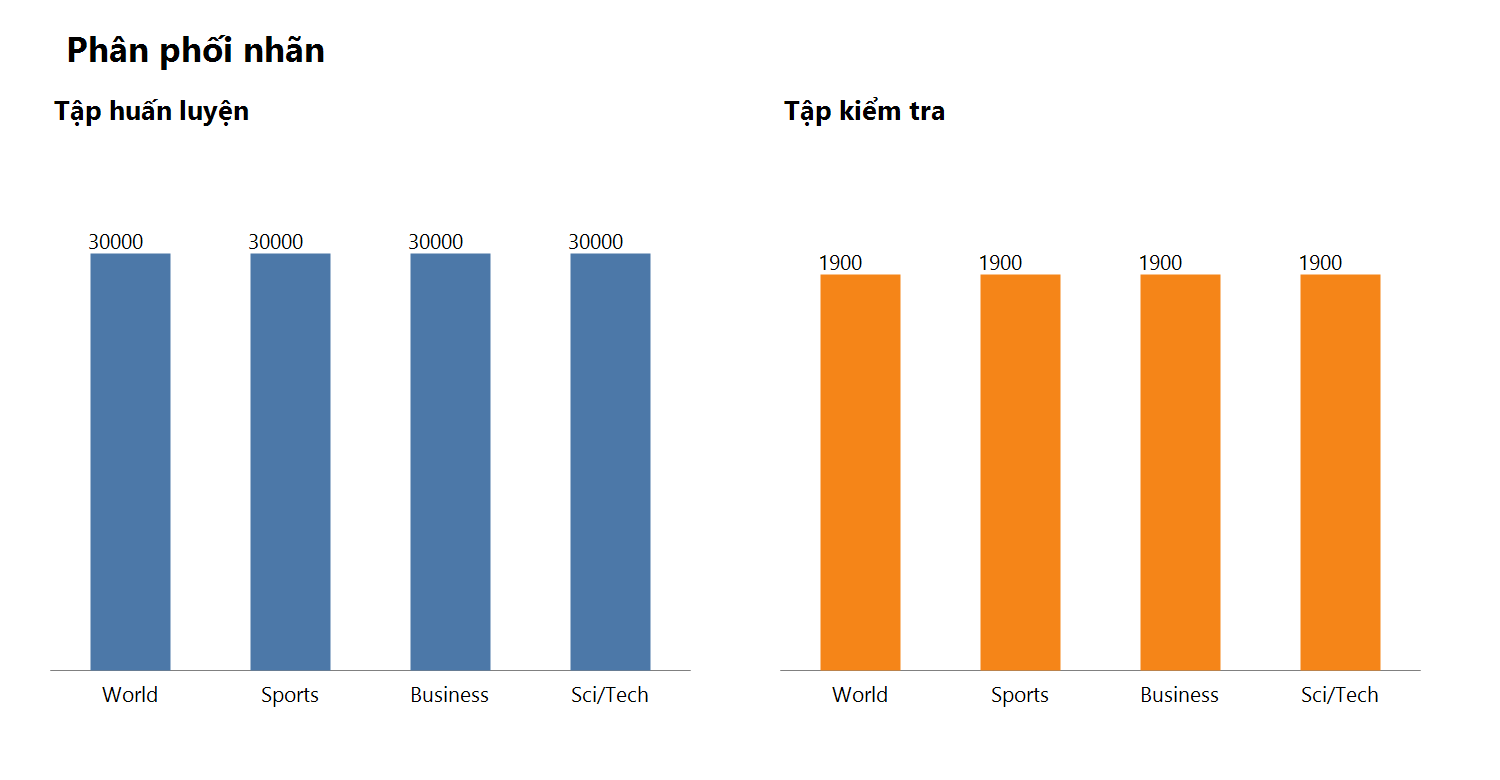
\includegraphics[width=0.92\textwidth,keepaspectratio]{graphics/class_distribution.png}
  \caption{Phân phối nhãn của tập huấn luyện (trái) và tập kiểm tra (phải). Hai biểu đồ dùng thang đo trục tung khác nhau.}
  \label{fig:label-distribution}
\end{figure}

Hình~\ref{fig:label-distribution} cho thấy số mẫu của bốn lớp bằng nhau trong cả tập huấn luyện và tập kiểm tra. Do mỗi lớp chiếm một phần tư số mẫu, phân phối nhãn thực nghiệm có dạng:

\begin{equation}
  \widehat{P}(Y=k)=\frac{1}{4},\qquad k\in\{1,2,3,4\}.
  \label{eq:uniform-label}
\end{equation}

Với phân phối này, nhóm không cần lấy mẫu lại hoặc điều chỉnh trọng số để khắc phục mất cân bằng lớp. Tuy nhiên, sự cân bằng về số lượng không hàm ý rằng các chủ đề có độ khó phân loại tương đương. Vì vậy, phần phân tích tiếp theo tập trung thêm vào đặc điểm của văn bản.

\section{Chuẩn bị dữ liệu và phân tích đặc trưng}

\subsection{Tạo văn bản đầu vào}

\firstparagraph Trong bước chuẩn bị dữ liệu, hàm \texttt{prepare\_dataset()} tạo trường \texttt{text} bằng cách nối nội dung \texttt{title} với \texttt{description}, theo thứ tự này và ngăn cách bằng một dấu cách. Tiếp đó, hàm \texttt{add\_class\_names()} ánh xạ giá trị nhãn số trong \texttt{class} (từ 1 đến 4) sang tên chủ đề tương ứng và lưu vào trường \texttt{class\_name}.

Sau hai thao tác này, dữ liệu có năm cột. Trường \texttt{text} chứa nội dung đầu vào để tiền xử lý và trích xuất đặc trưng. Trường \texttt{class} là nhãn đích. Trường \texttt{class\_name} chỉ dùng để hiển thị và diễn giải, và không được đưa vào mô hình.

\subsection{Thống kê độ dài văn bản}

\firstparagraph Hai đại lượng được khảo sát trên văn bản đã ghép, trước khi làm sạch: \texttt{text\_length} (số ký tự) và \texttt{word\_count} (số từ). Bảng~\ref{tab:text-length-statistics} trình bày đầy đủ thống kê của \textbf{120.000} mẫu huấn luyện.

\begin{table}[H]
  \centering
  \caption{Thống kê độ dài văn bản trên tập huấn luyện trước tiền xử lý}
  \label{tab:text-length-statistics}
  \small
  \renewcommand{\arraystretch}{1.15}
  \setlength{\tabcolsep}{18pt}
  \begin{tabular}{lrr}
    \toprule
    \textbf{Thống kê} & \textbf{Số ký tự} & \textbf{Số từ} \\
    & \texttt{text\_length} & \texttt{word\_count} \\
    \midrule
    Số mẫu (count)       & 120.000    & 120.000 \\
    Trung bình (mean)    & 236,460025 & 37,844617 \\
    Độ lệch chuẩn (std)  & 66,529799  & 10,088702 \\
    Nhỏ nhất (min)       & 17         & 4 \\
    Phân vị 25\% (Q1)   & 196        & 32 \\
    Trung vị 50\%       & 232        & 37 \\
    Phân vị 75\% (Q3)   & 266        & 43 \\
    Lớn nhất (max)       & 1.012      & 177 \\
    \bottomrule
  \end{tabular}
  \par\vspace{3pt}
  \parbox{0.82\textwidth}{\footnotesize\textit{Ghi chú:} Các thống kê được tính trên 120.000 văn bản huấn luyện sau khi ghép tiêu đề và mô tả, trước bước làm sạch.}
\end{table}

Trung bình mỗi văn bản có khoảng \textbf{236,46} ký tự và \textbf{37,84} từ, với độ lệch chuẩn lần lượt là 66,53 ký tự và 10,09 từ. Số từ trong bảng là tổng số lần xuất hiện của các từ. Đại lượng này khác với số từ duy nhất (unique words), vì mỗi từ chỉ được đếm một lần trong một văn bản khi tính số từ duy nhất.

Hình~\ref{fig:text-length-distribution} cho thấy phần lớn mẫu có độ dài ngắn, tương đương đoạn dẫn hoặc tóm tắt tin tức. Khoảng tứ phân vị có độ rộng $\mathrm{IQR}=Q3-Q1$ bằng \textbf{70} ký tự và \textbf{11} từ. Kết quả này cho thấy độ dài tập trung tương đối hẹp ở vùng trung tâm. Trung bình gần trung vị và hơi lớn hơn trung vị. Kết hợp với giá trị cực đại cao, các thống kê này gợi ý phân phối có đuôi phải do một số văn bản dài bất thường. Tuy nhiên, các thống kê trên chưa đủ để định lượng mức độ lệch.

Các mẫu rất ngắn có thể xuất hiện vì tiêu đề hoặc mô tả bị cắt, hoặc vì nhiễu trong dữ liệu. Nhóm cần kiểm tra trực tiếp các mẫu này trước khi kết luận. Nhóm không loại mẫu chỉ dựa vào độ dài nhỏ nhất hoặc lớn nhất.

\begin{figure}[H]
  \centering
  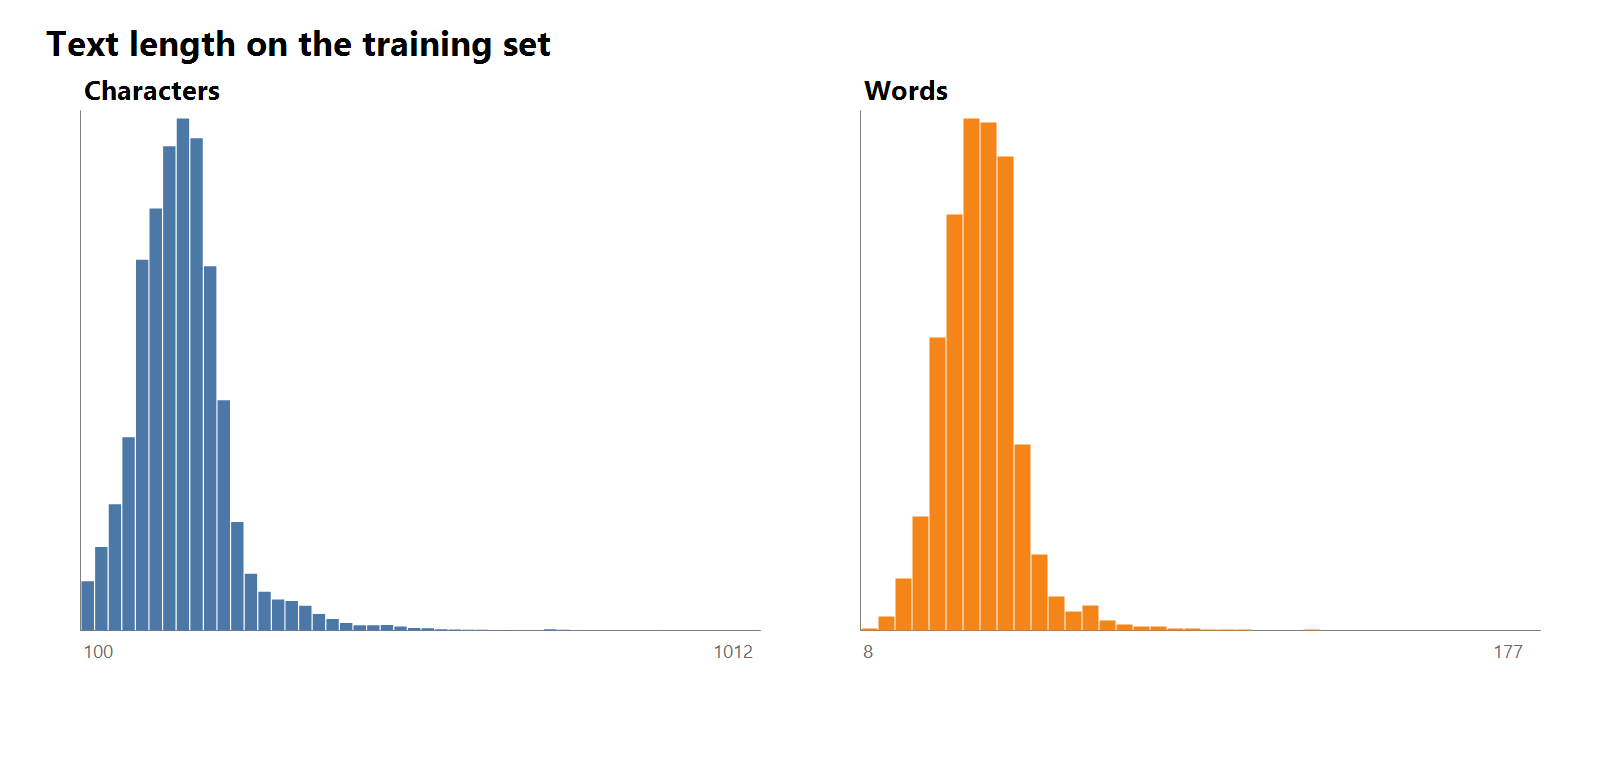
\includegraphics[width=0.92\textwidth,keepaspectratio]{graphics/text_length_distribution.png}
  \caption{Phân phối độ dài văn bản theo số ký tự (trái) và số từ (phải). Trục tung biểu thị số mẫu trong mỗi khoảng; phần lớn mẫu tập trung ở vùng độ dài ngắn, với đuôi phân phối kéo dài về bên phải.}
  \label{fig:text-length-distribution}
\end{figure}

\begin{figure}[H]
  \centering
  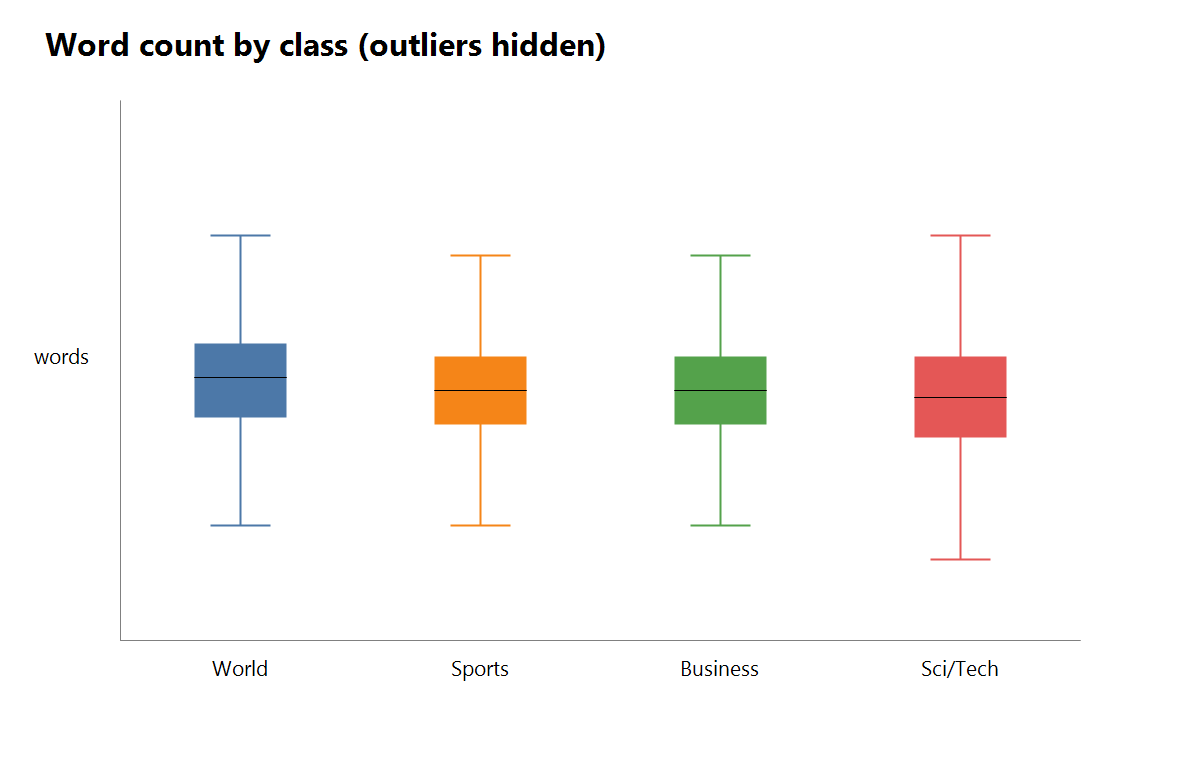
\includegraphics[width=0.78\textwidth,keepaspectratio]{graphics/text_length_by_class.png}
  \caption{Số từ theo từng chủ đề trên tập huấn luyện. Điểm ngoại lai không được vẽ để làm rõ vùng trung tâm. Trung vị lần lượt là \textbf{39} từ (World), \textbf{37} từ (Sports), \textbf{37} từ (Business) và \textbf{36} từ (Sci/Tech). Do đó, độ dài không phải tín hiệu phân biệt mạnh.}
  \label{fig:text-length-by-class}
\end{figure}

\subsection{Từ phổ biến và từ đặc trưng theo lớp}

\firstparagraph Trước khi loại stopword, các token chữ cái xuất hiện nhiều nhất là từ chức năng. Trên tập huấn luyện, từ \textit{the} xuất hiện \textbf{205.483} lần. Các từ tiếp theo là \textit{to}, \textit{a}, \textit{of}, \textit{in} và \textit{and}. Token \textit{s} cũng đứng cao vì dấu sở hữu cách bị tách thành một chữ cái riêng. Hình~\ref{fig:top-words-raw} giải thích vì sao lớp \texttt{TextPreprocessor} phải loại stopword: nếu nhóm giữ các từ này, biểu diễn Bag-of-Words sẽ bị chi phối bởi những từ xuất hiện ở mọi chủ đề.

\begin{figure}[H]
  \centering
  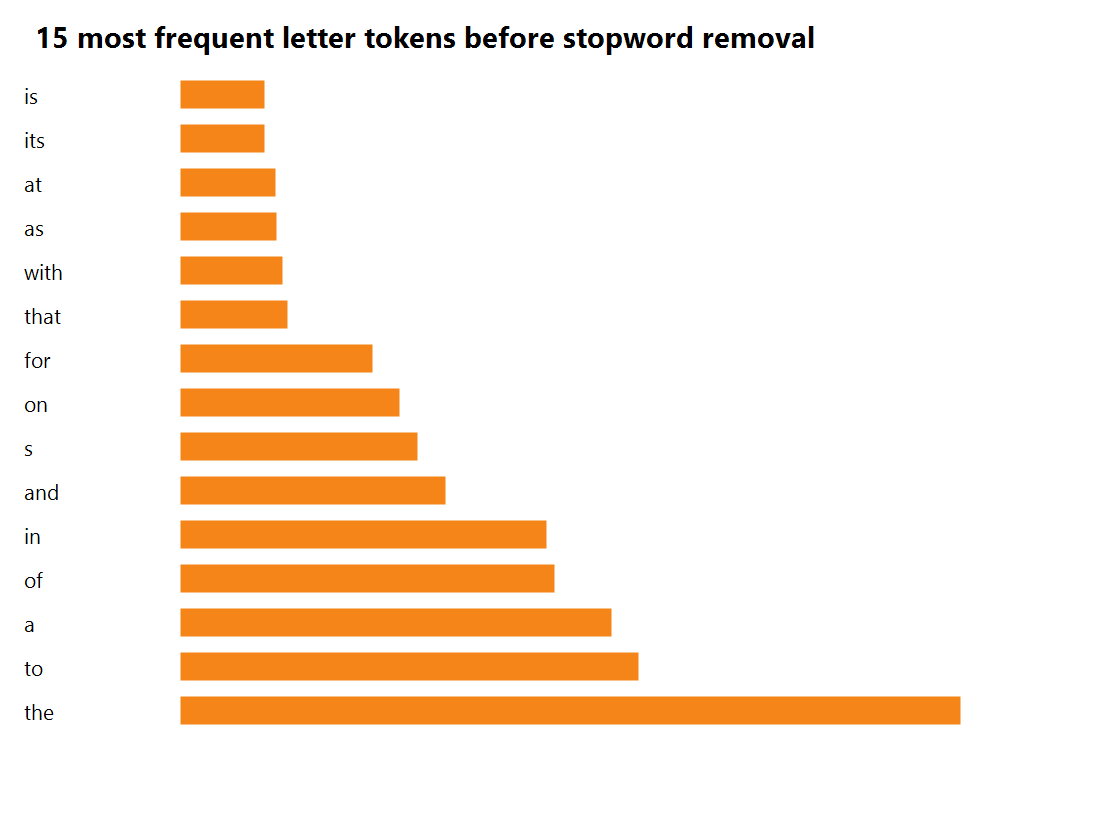
\includegraphics[width=0.78\textwidth,keepaspectratio]{graphics/top_words_raw.png}
  \caption{Mười lăm token chữ cái xuất hiện nhiều nhất trên văn bản đã ghép, trước khi loại stopword.}
  \label{fig:top-words-raw}
\end{figure}

Hình~\ref{fig:top-words-by-class} trình bày các từ xuất hiện nhiều nhất trong từng lớp sau khi văn bản được chuyển về chữ thường, loại URL, lọc để chỉ giữ chữ cái và bỏ stopword tiếng Anh. Với lớp World, các từ nổi bật là \textit{\textbf{iraq}} và \textit{president}. Với lớp Sports, các từ nổi bật là \textit{\textbf{game}}, \textit{season}, \textit{team} và \textit{win}. Với lớp Business, các từ nổi bật là \textit{\textbf{oil}}, \textit{stocks}, \textit{inc} và \textit{\textbf{company}}. Với lớp Sci/Tech, các từ thường gặp là \textit{\textbf{microsoft}}, \textit{software} và \textit{internet}. Từ \textit{\textbf{company}} xuất hiện trong cả Business và Sci/Tech, nên hai lớp có một phần từ vựng chung. Sự chồng lấn này có thể làm tăng khả năng mô hình nhầm lẫn giữa hai lớp.

Sau các bước lọc, một số token không phản ánh chủ đề vẫn còn trong văn bản. Các token \textit{reuters}, \textit{ap} và \textit{afp} là tên hãng tin. Các token \textit{gt} và \textit{lt} phát sinh từ thực thể HTML \texttt{\&gt;} và \texttt{\&lt;}. Khi dấu câu và ký tự đặc biệt bị loại bỏ, phần chữ trong thực thể vẫn còn lại. Tương tự, token \texttt{dwindlingband} trong ví dụ tiền xử lý hình thành khi dấu gạch chéo ngược bị xóa mà không được thay bằng khoảng trắng. Đây là các dạng nhiễu từ dữ liệu thu thập, và pipeline hiện tại chưa xử lý riêng các trường hợp này.

\begin{figure}[H]
  \centering
  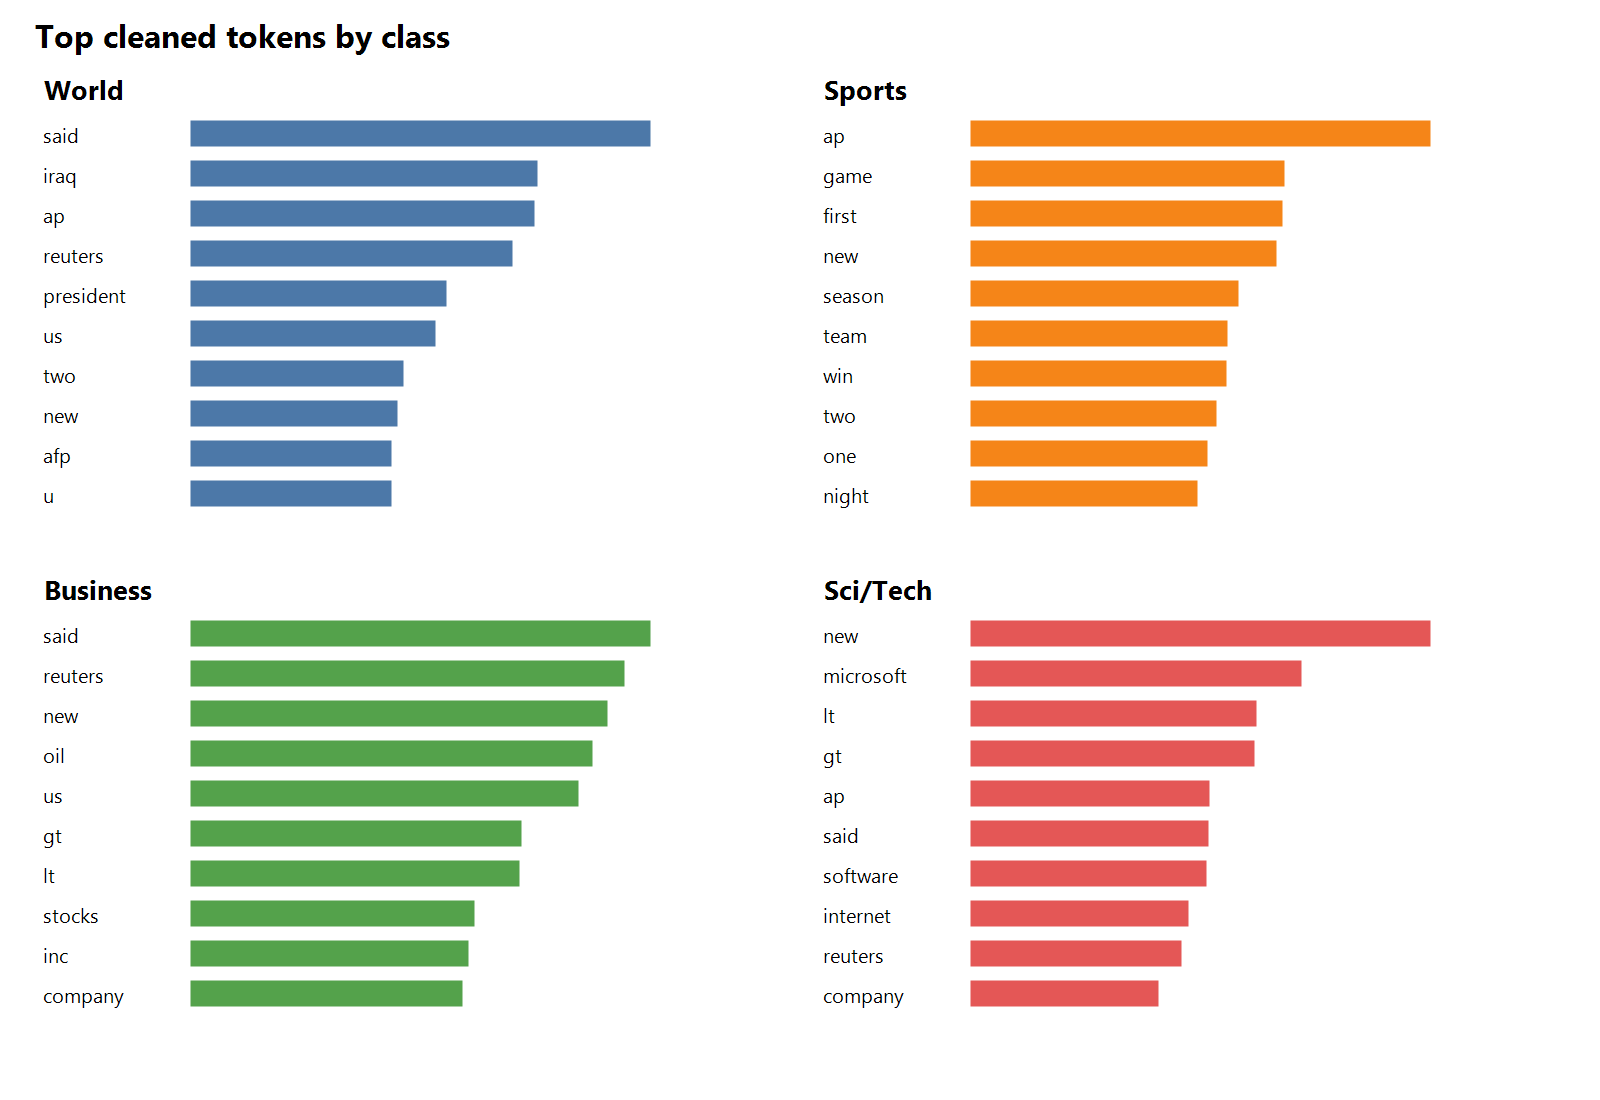
\includegraphics[width=0.92\textwidth,keepaspectratio]{graphics/top_words_by_class.png}
  \caption{Mười token xuất hiện nhiều nhất trong từng lớp sau khi bỏ stopword. Bước lemmatization chưa được áp dụng trên hình này.}
  \label{fig:top-words-by-class}
\end{figure}

\section{Pipeline học máy truyền thống}

\firstparagraph Tập gốc gồm 120.000 mẫu huấn luyện và 7.600 mẫu kiểm tra, được chia đều cho bốn lớp World, Sports, Business và Sci/Tech. Nhãn gốc nhận giá trị trong $\{1,2,3,4\}$. Sau khi tiền xử lý, nhóm chia tập huấn luyện thành 102.000 mẫu train và 18.000 mẫu validation. Trường đầu vào được tạo theo công thức:

\begin{equation}
  \texttt{text}=\texttt{title}+\texttt{" "}+\texttt{description}.
  \label{eq:combine-text}
\end{equation}

Việc giữ phép chia chính thức train/test giúp kết quả có thể đối chiếu với các nghiên cứu dùng AG News. Tập validation chỉ được lấy từ phần train. Bộ vector hóa, trọng số IDF và siêu tham số không được học từ tập kiểm tra.

\subsection{Tiền xử lý dữ liệu}

\firstparagraph Văn bản tin tức thô chứa chữ hoa/thường không thống nhất, URL, ký tự đặc biệt, số liệu và các token ít mang tín hiệu chủ đề. Lớp \texttt{TextPreprocessor} đóng gói một chuỗi xử lý xác định và áp dụng chuỗi xử lý này giống nhau cho tập huấn luyện lẫn tập kiểm tra:

\begin{enumerate}[leftmargin=2em,itemsep=5pt]
  \item \textbf{Kết hợp tiêu đề và mô tả.} Tiêu đề thường chứa từ khóa chủ đề, còn mô tả bổ sung ngữ cảnh. Văn bản sau khi nối có trung bình khoảng 236 ký tự và 38 từ.
  \item \textbf{Chuẩn hóa chữ thường.} Các biến thể như \textit{Reuters} và \textit{reuters} được đưa về cùng một token, tránh làm loãng thống kê.
  \item \textbf{Loại URL.} Biểu thức chính quy \texttt{http\string\\S+|www\string\\S+} xóa đường dẫn, vốn thường tạo nhiều token hiếm và ít hữu ích cho phân loại chủ đề.
  \item \textbf{Chỉ giữ chữ cái tiếng Anh.} Mẫu \texttt{[\string^a-zA-Z\string\\s]} loại chữ số, dấu câu, ký hiệu tiền tệ và dấu gạch ngang. Quyết định này giảm từ vựng hiếm nhưng đồng thời có thể làm mất tín hiệu như giá cổ phiếu hoặc tỷ số thể thao.
  \item \textbf{Chuẩn hóa khoảng trắng.} Lệnh tương đương \texttt{re.sub(r'\string\\s+', ' ', text)} gộp các khoảng trắng liên tiếp và loại khoảng trắng thừa ở hai đầu.
  \item \textbf{Tách từ.} Hàm \texttt{nltk.word\_tokenize} chuyển chuỗi thành danh sách token.
  \item \textbf{Loại stopword tiếng Anh.} Các từ chức năng phổ biến trong danh sách NLTK được bỏ để giảm số chiều và hạn chế BoW bị chi phối bởi từ xuất hiện ở mọi lớp.
  \item \textbf{Lemmatization.} \texttt{WordNetLemmatizer} đưa các biến thể như \textit{bears} về \textit{bear}. Do không gắn nhãn từ loại, lemmatizer mặc định thiên về danh từ và có thể không chuẩn hóa triệt để một số động từ.
  \item \textbf{Ghép lại văn bản.} Các token còn lại được nối bằng một dấu cách và lưu trong cột \texttt{cleaned\_text}.
\end{enumerate}

Ví dụ dưới đây lấy từ mẫu đầu tiên của tập huấn luyện:

\begin{quote}\small
\setlength{\fboxsep}{7pt}
\noindent\colorbox{ucRule!12}{%
  \parbox{\dimexpr\linewidth-2\fboxsep\relax}{%
    \raggedright
    \textbf{\textcolor{ucRule!85!black}{Gốc}}\par
    \textit{Wall St. Bears Claw Back Into the Black (Reuters) Reuters -- Short-sellers, Wall Street's dwindling\textbackslash band of ultra-cynics, are seeing green again.}%
  }%
}
\par\vspace{5pt}
\noindent\colorbox{ucRule!12}{%
  \parbox{\dimexpr\linewidth-2\fboxsep\relax}{%
    \raggedright
    \textbf{\textcolor{ucRule!85!black}{Sau tiền xử lý}}\par
    \texttt{wall st bear claw back black reuters reuters shortsellers wall street dwindlingband ultracynics seeing green}%
  }%
}
\end{quote}

Kết quả cho thấy quá trình chữ thường hóa, loại stopword và chuẩn hóa \textit{bears} thành \textit{bear} đã được thực hiện. Token \texttt{dwindlingband} cũng cho thấy một nhiễu còn lại: chuỗi escape từ dữ liệu thu thập bị dính vào từ đứng trước. Nhóm có thể cải thiện bước này bằng quy tắc xử lý chuỗi escape trước khi lọc ký tự.

\begin{figure}[H]
  \centering
  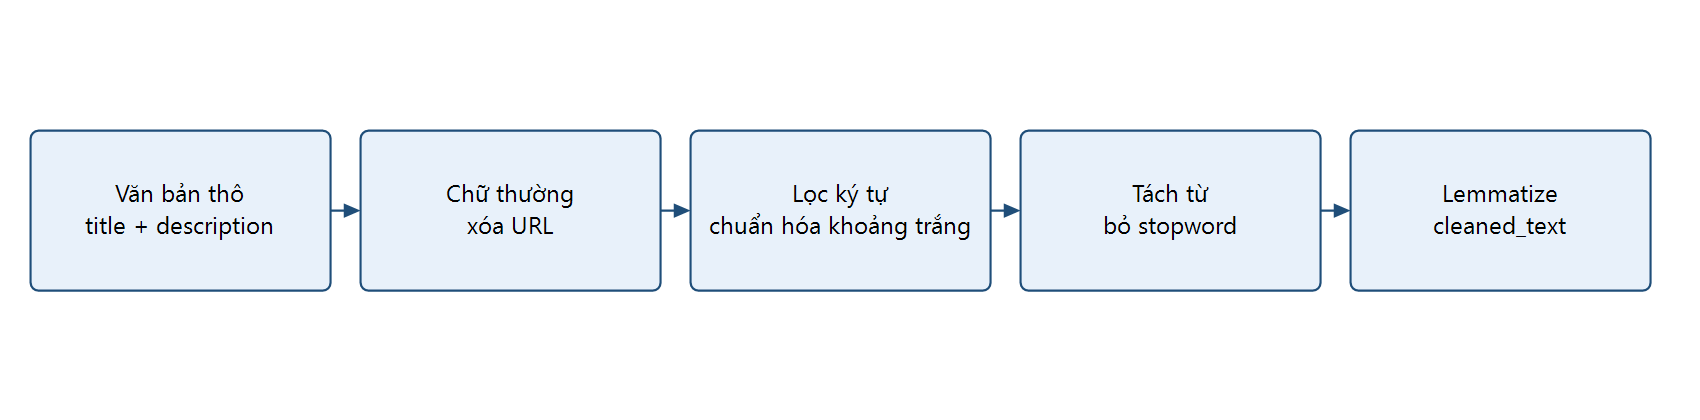
\includegraphics[width=\textwidth,keepaspectratio]{graphics/preprocessing_pipeline.png}
  \caption{Chuỗi tiền xử lý văn bản của pipeline học máy truyền thống.}
  \label{fig:preprocessing-pipeline}
\end{figure}

Đầu ra của giai đoạn này gồm văn bản đã làm sạch, các ma trận BoW/TF--IDF cho train/validation/test và các vector nhãn tương ứng. Bộ vector hóa chỉ được \texttt{fit} trên phần train (102.000 mẫu). Các tập validation và test chỉ được \texttt{transform}. Nếu nhóm dùng kiểm định chéo, bộ vector hóa phải được học lại trong từng fold để tránh rò rỉ dữ liệu.

\subsection{Trích xuất đặc trưng}

\subsubsection{Bag-of-Words}

\firstparagraph Với từ vựng $V$ gồm tối đa 5.000 từ thường gặp nhất trên phần train, Count Vectorizer biểu diễn văn bản $d_i$ bằng số lần xuất hiện của mỗi từ:

\begin{equation}
  x_{i,j}=c(v_j,d_i),\qquad j=1,\ldots,|V|.
  \label{eq:bow}
\end{equation}

Biểu diễn BoW đơn giản, dễ diễn giải và phù hợp với Multinomial Naive Bayes. Tuy nhiên, biểu diễn này không giữ thứ tự từ, không chuẩn hóa độ dài văn bản và có thể để các từ phổ biến như \textit{reuters}, \textit{said}, \textit{year} lấn át từ khóa phân biệt.

\subsubsection{TF--IDF}

\firstparagraph TF--IDF (Term Frequency--Inverse Document Frequency) đánh giá mức độ quan trọng của một từ dựa trên số lần xuất hiện của từ đó trong văn bản và độ phổ biến của từ trong toàn bộ phần train \cite{salton1988tfidf,manning2008ir}. Trong báo cáo này, vectorizer của scikit-learn dùng công thức IDF có làm trơn:

\begin{align}
  \mathrm{IDF}(t)&=\ln\!\left(\frac{1+N}{1+\mathrm{DF}(t)}\right)+1,\label{eq:idf}\\
  \mathrm{TF\mbox{-}IDF}(t,d)&=\mathrm{TF}(t,d)\,\mathrm{IDF}(t),\label{eq:tfidf}
\end{align}

trong đó $N=102.000$ là số văn bản dùng để \texttt{fit} vectorizer (phần train) và $\mathrm{DF}(t)$ là số văn bản train có chứa từ $t$. Sau khi tính TF--IDF, mỗi vector văn bản được chuẩn hóa theo chuẩn $L_2$. Vì vậy, từ xuất hiện trong hầu hết văn bản có IDF thấp, còn những từ mang tính chủ đề hơn, chẳng hạn \textit{olympic}, \textit{nasdaq}, \textit{nasa} hoặc \textit{iraq}, thường có IDF cao hơn.

Ở bước trích xuất đặc trưng, cả hai vectorizer đều dùng unigram và giới hạn từ vựng ở \texttt{max\_features=5000}. Các tham số còn lại được giữ theo mặc định của scikit-learn. Vì văn bản đã được chuyển về chữ thường trong bước tiền xử lý, thiết lập \texttt{lowercase} mặc định của vectorizer không làm phát sinh thêm biến thể hoa/thường. Giới hạn 5.000 đặc trưng giúp cân bằng độ phủ từ vựng với thời gian huấn luyện, đồng thời hạn chế việc mô hình phụ thuộc vào các từ quá hiếm. Module \texttt{experiments/feature\_selection.py} hỗ trợ các phương pháp chọn đặc trưng như kiểm định Chi-bình phương ($\chi^2$), Mutual Information và \texttt{SelectFromModel}, nhưng các thí nghiệm chính không áp dụng bước này. Nhờ đó, việc so sánh tập trung vào hiệu quả của BoW và TF--IDF.

\begin{table}[H]
  \centering
  \caption{Kích thước các ma trận đặc trưng thực nghiệm}
  \label{tab:feature-matrices}
  \small
  \renewcommand{\arraystretch}{1.15}
  \begin{tabular}{lccc}
    \toprule
    \textbf{Biểu diễn} & \textbf{Train} & \textbf{Validation} & \textbf{Test} \\
    \midrule
    TF--IDF & $102.000\times5.000$ & $18.000\times5.000$ & $7.600\times5.000$ \\
    BoW     & $102.000\times5.000$ & $18.000\times5.000$ & $7.600\times5.000$ \\
    \bottomrule
  \end{tabular}
\end{table}

Các ma trận được lưu ở dạng thưa trong \texttt{data/processed/}. Hai bộ vector hóa đã khớp được lưu tại \texttt{models/tfidf\_vectorizer.pkl} và \texttt{models/count\_vectorizer.pkl} để tái sử dụng khi suy luận.

\subsection{Huấn luyện và đánh giá mô hình}

\subsubsection{Thiết kế thí nghiệm}

\firstparagraph Nhóm huấn luyện đầy đủ sáu tổ hợp tạo bởi hai cách biểu diễn $\{\text{BoW},\text{TF--IDF}\}$ và ba mô hình $\{\text{Multinomial NB},\text{Logistic Regression},\text{Linear SVM}\}$. Sáu tổ hợp được huấn luyện trên 102.000 mẫu train và được so sánh trên 18.000 mẫu validation. Sau đó, mô hình tốt nhất được đánh giá một lần trên 7.600 mẫu test. Tham số \texttt{random\_state=42} được cố định khi thuật toán hỗ trợ tham số này. Thiết kế thí nghiệm cho phép so sánh thuật toán khi cố định đặc trưng, đồng thời so sánh đặc trưng khi cố định thuật toán.

Nhóm không dùng Kernel SVM vì chi phí tính toán cao trên khoảng 100.000 mẫu và 5.000 chiều. Các mô hình Random Forest, Decision Tree và Gradient Boosting có sẵn trong \texttt{TraditionalMLModels} nhưng không thuộc thí nghiệm chính, vì chúng thường kém phù hợp hơn mô hình tuyến tính trên dữ liệu văn bản rất thưa. SVM tuyến tính dựa trên nguyên lý cực đại hóa lề phân lớp \cite{cortes1995svm}.

\subsubsection{Cơ sở toán học các mô hình và thiết lập siêu tham số}

\firstparagraph Nhóm lựa chọn ba mô hình học máy truyền thống đại diện cho các trường phái khác nhau: mô hình cơ sở xác suất (Multinomial Naive Bayes), mô hình phân loại tuyến tính xác suất (Logistic Regression), và mô hình tối ưu hóa biên lề cực đại (Linear SVM). Cả ba mô hình đều được xây dựng để xử lý dữ liệu ma trận thưa nhiều chiều với chi phí tính toán thấp.

\begin{enumerate}[leftmargin=2em,itemsep=6pt]
  \item \textbf{Multinomial Naive Bayes (MNB):} Mô hình dựa trên định lý xác suất Bayes với giả thiết độc lập có điều kiện giữa các đặc trưng từ vựng:
  \begin{equation}
    P(Y=k \mid \mathbf{x}) = \frac{P(Y=k) P(\mathbf{x} \mid Y=k)}{P(\mathbf{x})} \propto P(Y=k) \prod_{j=1}^{|V|} P(w_j \mid Y=k)^{x_j},
    \label{eq:nb-posterior}
  \end{equation}
  trong đó $x_j$ là số lần xuất hiện (hoặc trọng số TF--IDF) của từ vựng $w_j$, và $|V| = 5.000$ là kích thước từ vựng. Xác suất hợp lý $P(w_j \mid Y=k) = \theta_{k,j}$ được ước lượng bằng kỹ thuật làm trơn Laplace (Laplace smoothing với $\alpha=1{,}0$):
  \begin{equation}
    \hat{\theta}_{k,j} = \frac{N_{k,j} + \alpha}{N_k + \alpha |V|},
    \label{eq:nb-laplace}
  \end{equation}
  với $N_{k,j}$ là tổng tần suất từ $w_j$ trong lớp $k$, và $N_k = \sum_{j=1}^{|V|} N_{k,j}$. Để tránh hiện tượng tràn số dưới (underflow), quy tắc quyết định lớp được tính trong không gian log:
  \begin{equation}
    \hat{y} = \arg\max_{k \in \{1,2,3,4\}} \left[ \ln P(Y=k) + \sum_{j=1}^{|V|} x_j \ln \hat{\theta}_{k,j} \right].
    \label{eq:nb-decision}
  \end{equation}

  \item \textbf{Logistic Regression (Softmax Regression):} Với bài toán phân loại bốn chủ đề ($K=4$), mô hình xấp xỉ phân phối xác suất hậu nghiệm thông qua hàm kích hoạt Softmax:
  \begin{equation}
    P(Y=k \mid \mathbf{x}) = \frac{\exp(\mathbf{w}_k^T \mathbf{x} + b_k)}{\sum_{c=1}^K \exp(\mathbf{w}_c^T \mathbf{x} + b_c)},
    \label{eq:softmax}
  \end{equation}
  trong đó $\mathbf{w}_k \in \mathbb{R}^{|V|}$ là vector trọng số và $b_k \in \mathbb{R}$ là hệ số điều chỉnh (bias) cho lớp $k$. Quá trình huấn luyện giải bài toán tối thiểu hóa hàm mất mát Cross-Entropy kết hợp điều chuẩn $L_2$:
  \begin{equation}
    \min_{\mathbf{W}, \mathbf{b}} \left\{ -\frac{1}{N} \sum_{i=1}^N \sum_{k=1}^K \mathbb{I}(y_i = k) \ln P(Y=k \mid \mathbf{x}_i) + \frac{1}{2C} \sum_{k=1}^K \|\mathbf{w}_k\|_2^2 \right\},
    \label{eq:logreg-loss}
  \end{equation}
  với $\mathbb{I}(\cdot)$ là hàm chỉ thị. Siêu tham số phạt nghịch đảo $C=1{,}0$ kiểm soát độ mạnh của điều chuẩn, hạn chế hiện tượng quá khớp (overfitting) trên các từ hiếm. Nhóm cấu hình \texttt{max\_iter=1000} và tận dụng tính toán song song \texttt{n\_jobs=-1}.

  \item \textbf{Linear Support Vector Machine (Linear SVM):} Triển khai qua \texttt{LinearSVC} dựa trên thư viện LibLinear theo chiến lược One-vs-Rest (OvR). Với từng lớp $k$, mô hình tìm siêu phẳng phân tách $(\mathbf{w}_k, b_k)$ cực đại hóa lề phân lớp với hàm mất mát Hinge mềm (Soft-margin Hinge Loss):
  \begin{equation}
    \min_{\mathbf{w}_k, b_k, \boldsymbol{\xi}} \left\{ \frac{1}{2} \|\mathbf{w}_k\|_2^2 + C \sum_{i=1}^N \xi_i \right\}
    \label{eq:svm-obj}
  \end{equation}
  thỏa mãn ràng buộc:
  \begin{equation}
    y_{i,k} (\mathbf{w}_k^T \mathbf{x}_i + b_k) \ge 1 - \xi_i, \quad \xi_i \ge 0, \quad \forall i=1,\ldots,N,
    \label{eq:svm-constraint}
  \end{equation}
  trong đó $y_{i,k} \in \{+1, -1\}$ (gán $+1$ nếu mẫu $i$ thuộc lớp $k$, ngược lại gán $-1$), và $\xi_i$ là biến bù (slack variable) đo mức vi phạm lề. Hàm quyết định đa lớp là:
  \begin{equation}
    \hat{y} = \arg\max_{k \in \{1,2,3,4\}} (\mathbf{w}_k^T \mathbf{x} + b_k).
    \label{eq:svm-decision}
  \end{equation}
  Siêu tham số $C=1{,}0$ và \texttt{max\_iter=1000} mang lại sự cân bằng tối ưu giữa việc mở rộng lề và giới hạn sai số phân lớp.
\end{enumerate}

Các mô hình được huấn luyện bằng các cấu hình tham số mặc định chuẩn của Machine Learning ($C=1{,}0$ đối với Linear SVM và Logistic Regression, $\alpha=1{,}0$ với làm trơn Laplace ở Multinomial Naive Bayes). Việc giữ cố định các siêu tham số tiêu chuẩn này nhằm so sánh công bằng, khách quan hiệu năng bản chất giữa các thuật toán trên cùng hai không gian đặc trưng BoW và TF--IDF.

\subsubsection{Độ đo đánh giá và cơ sở lựa chọn}

\firstparagraph Do bộ dữ liệu AG News có phân phối hoàn toàn cân bằng (\textbf{25\%} mỗi lớp trên cả 120.000 mẫu train và 7.600 mẫu test), độ chính xác tổng thể (Accuracy) là độ đo phản ánh trung thực năng lực của mô hình:
\begin{equation}
  \mathrm{Accuracy} = \frac{\sum_{k=1}^K \mathrm{TP}_k}{N_{\text{total}}},
  \label{eq:accuracy}
\end{equation}
trong đó $\mathrm{TP}_k$ là số lượng mẫu dự đoán đúng của lớp $k$, và $N_{\text{total}}$ là tổng số mẫu đánh giá.

Tuy nhiên, Accuracy chỉ cung cấp bức tranh tổng quát mà không phản ánh được mức độ sai sót cục bộ giữa từng chủ đề tin tức. Do đó, nhóm sử dụng thêm Precision, Recall và F1-Score theo từng lớp:
\begin{align}
  \mathrm{Precision}_k &= \frac{\mathrm{TP}_k}{\mathrm{TP}_k + \mathrm{FP}_k}, \label{eq:precision}\\
  \mathrm{Recall}_k &= \frac{\mathrm{TP}_k}{\mathrm{TP}_k + \mathrm{FN}_k}, \label{eq:recall}\\
  \mathrm{F1}_k &= \frac{2 \cdot \mathrm{Precision}_k \cdot \mathrm{Recall}_k}{\mathrm{Precision}_k + \mathrm{Recall}_k}, \label{eq:f1-score}
\end{align}
với $\mathrm{FP}_k$ là số mẫu lớp khác bị dự đoán nhầm thành lớp $k$ (False Positive), và $\mathrm{FN}_k$ là số mẫu thật của lớp $k$ bị gán sai nhãn (False Negative).

Để đánh giá tổng hợp trên toàn bộ $K=4$ chủ đề, nhóm sử dụng chỉ số Macro-F1:
\begin{equation}
  \mathrm{Macro\mbox{-}F1} = \frac{1}{K} \sum_{k=1}^K \mathrm{F1}_k.
  \label{eq:macro-f1}
\end{equation}
Chỉ số Macro-F1 gán trọng số bình đẳng $\frac{1}{4}$ cho từng lớp, ngăn ngừa trường hợp mô hình tối ưu thiên vị cho một lớp riêng biệt mà làm suy giảm chất lượng phân loại ở các lớp còn lại. Đại lượng Weighted-F1 được định nghĩa là $\sum_{k=1}^K \frac{N_k}{N_{\text{total}}} \mathrm{F1}_k$; vì $N_k / N_{\text{total}} = 0{,}25$, giá trị Weighted-F1 thực nghiệm luôn tiệm cận Macro-F1, đóng vai trò kiểm chứng chéo tính nhất quán toán học.

Bên cạnh các chỉ số phân lớp, nhóm ghi nhận thời gian huấn luyện (\textit{train time}) và thời gian suy luận (\textit{predict time}) trong hàm \texttt{train\_and\_evaluate()} thuộc module \texttt{src/\allowbreak evaluation.py} để đo lường độ trễ tính toán. Ma trận nhầm lẫn (Confusion Matrix) được trực quan hóa nhằm chỉ ra rõ các cặp lớp có sự giao thoa ngữ nghĩa cao như Business--Sci/Tech.

\subsubsection{Kết quả trên tập validation}

\begin{landscape}
\begin{table}[H]
  \centering
  \caption{Kết quả sáu tổ hợp đặc trưng và mô hình trên 18.000 mẫu validation}
  \label{tab:traditional-results}
  \footnotesize
  \renewcommand{\arraystretch}{1.12}
  \setlength{\tabcolsep}{5pt}
  \begin{tabular}{llrrrrrrr}
    \toprule
    \textbf{Mô hình} & \textbf{Đặc trưng} & \textbf{Acc.} & \textbf{Prec. macro} & \textbf{Rec. macro} & \textbf{F1 macro} & \textbf{F1 weighted} & \textbf{Train (s)} & \textbf{Predict (s)} \\
    \midrule
    Naive Bayes         & BoW     & 0,8987 & 0,8983 & 0,8987 & 0,8984 & 0,8984 & 0,02 & 0,003 \\
    Logistic Regression & BoW     & 0,9028 & 0,9026 & 0,9028 & 0,9026 & 0,9026 & 1,90 & 0,003 \\
    Linear SVM          & BoW     & 0,9040 & 0,9039 & 0,9040 & 0,9038 & 0,9038 & 7,17 & 0,002 \\
    Naive Bayes         & TF--IDF & 0,8990 & 0,8987 & 0,8990 & 0,8987 & 0,8987 & 0,01 & 0,002 \\
    Logistic Regression & TF--IDF & 0,9127 & 0,9126 & 0,9127 & 0,9125 & 0,9125 & 1,89 & 0,001 \\
    Linear SVM          & TF--IDF & \textbf{0,9138} & \textbf{0,9137} & \textbf{0,9138} & \textbf{0,9136} & \textbf{0,9136} & \textbf{2,79} & 0,003 \\
    \bottomrule
  \end{tabular}
  \par\vspace{3pt}
  \parbox{0.95\textwidth}{\footnotesize\textit{Ghi chú:} Số liệu lấy từ \texttt{results/comparison.csv} (notebook 03). Mô hình tốt nhất sau đó được đánh giá trên tập test ở Mục~\ref{sec:error-analysis}.}
\end{table}
\end{landscape}

Mọi tổ hợp đều đạt từ khoảng 89,9\% accuracy và F1 trở lên. Các kết quả này cao hơn rõ rệt đường cơ sở dự đoán ngẫu nhiên hoặc luôn dự đoán một lớp (\textbf{25\%}). Accuracy, macro-F1 và weighted-F1 chênh nhau dưới 0,002 ở mọi cấu hình. Điều này phù hợp với phân bố nhãn cân bằng. Mô hình tốt nhất trên tập validation là Linear SVM kết hợp TF--IDF. Cấu hình này đạt accuracy 91,38\% và macro-F1 91,36\%, với thời gian huấn luyện khoảng 2,79 giây.

\subsection{So sánh trực quan và phân tích kết quả}

\subsubsection{So sánh theo thuật toán}

\firstparagraph Trên BoW, thứ tự accuracy là Linear SVM (0,9040), Logistic Regression (0,9028) và Naive Bayes (0,8987). Trên TF--IDF, thứ tự không đổi với các giá trị accuracy tương ứng 0,9138; 0,9127 và 0,8990. Linear SVM đứng đầu ở cả hai cách biểu diễn. Kết quả này phù hợp với đặc điểm dữ liệu văn bản thưa, nhiều chiều và thường gần phân tách tuyến tính.

Logistic Regression tiến sát SVM khi dùng TF--IDF và chỉ kém khoảng 0,11 điểm phần trăm accuracy. Naive Bayes gần như không cải thiện khi đổi BoW sang TF--IDF, vì trọng số TF--IDF không còn tuân theo diễn giải đếm multinomial nguyên thủy.

\begin{figure}[H]
  \centering
  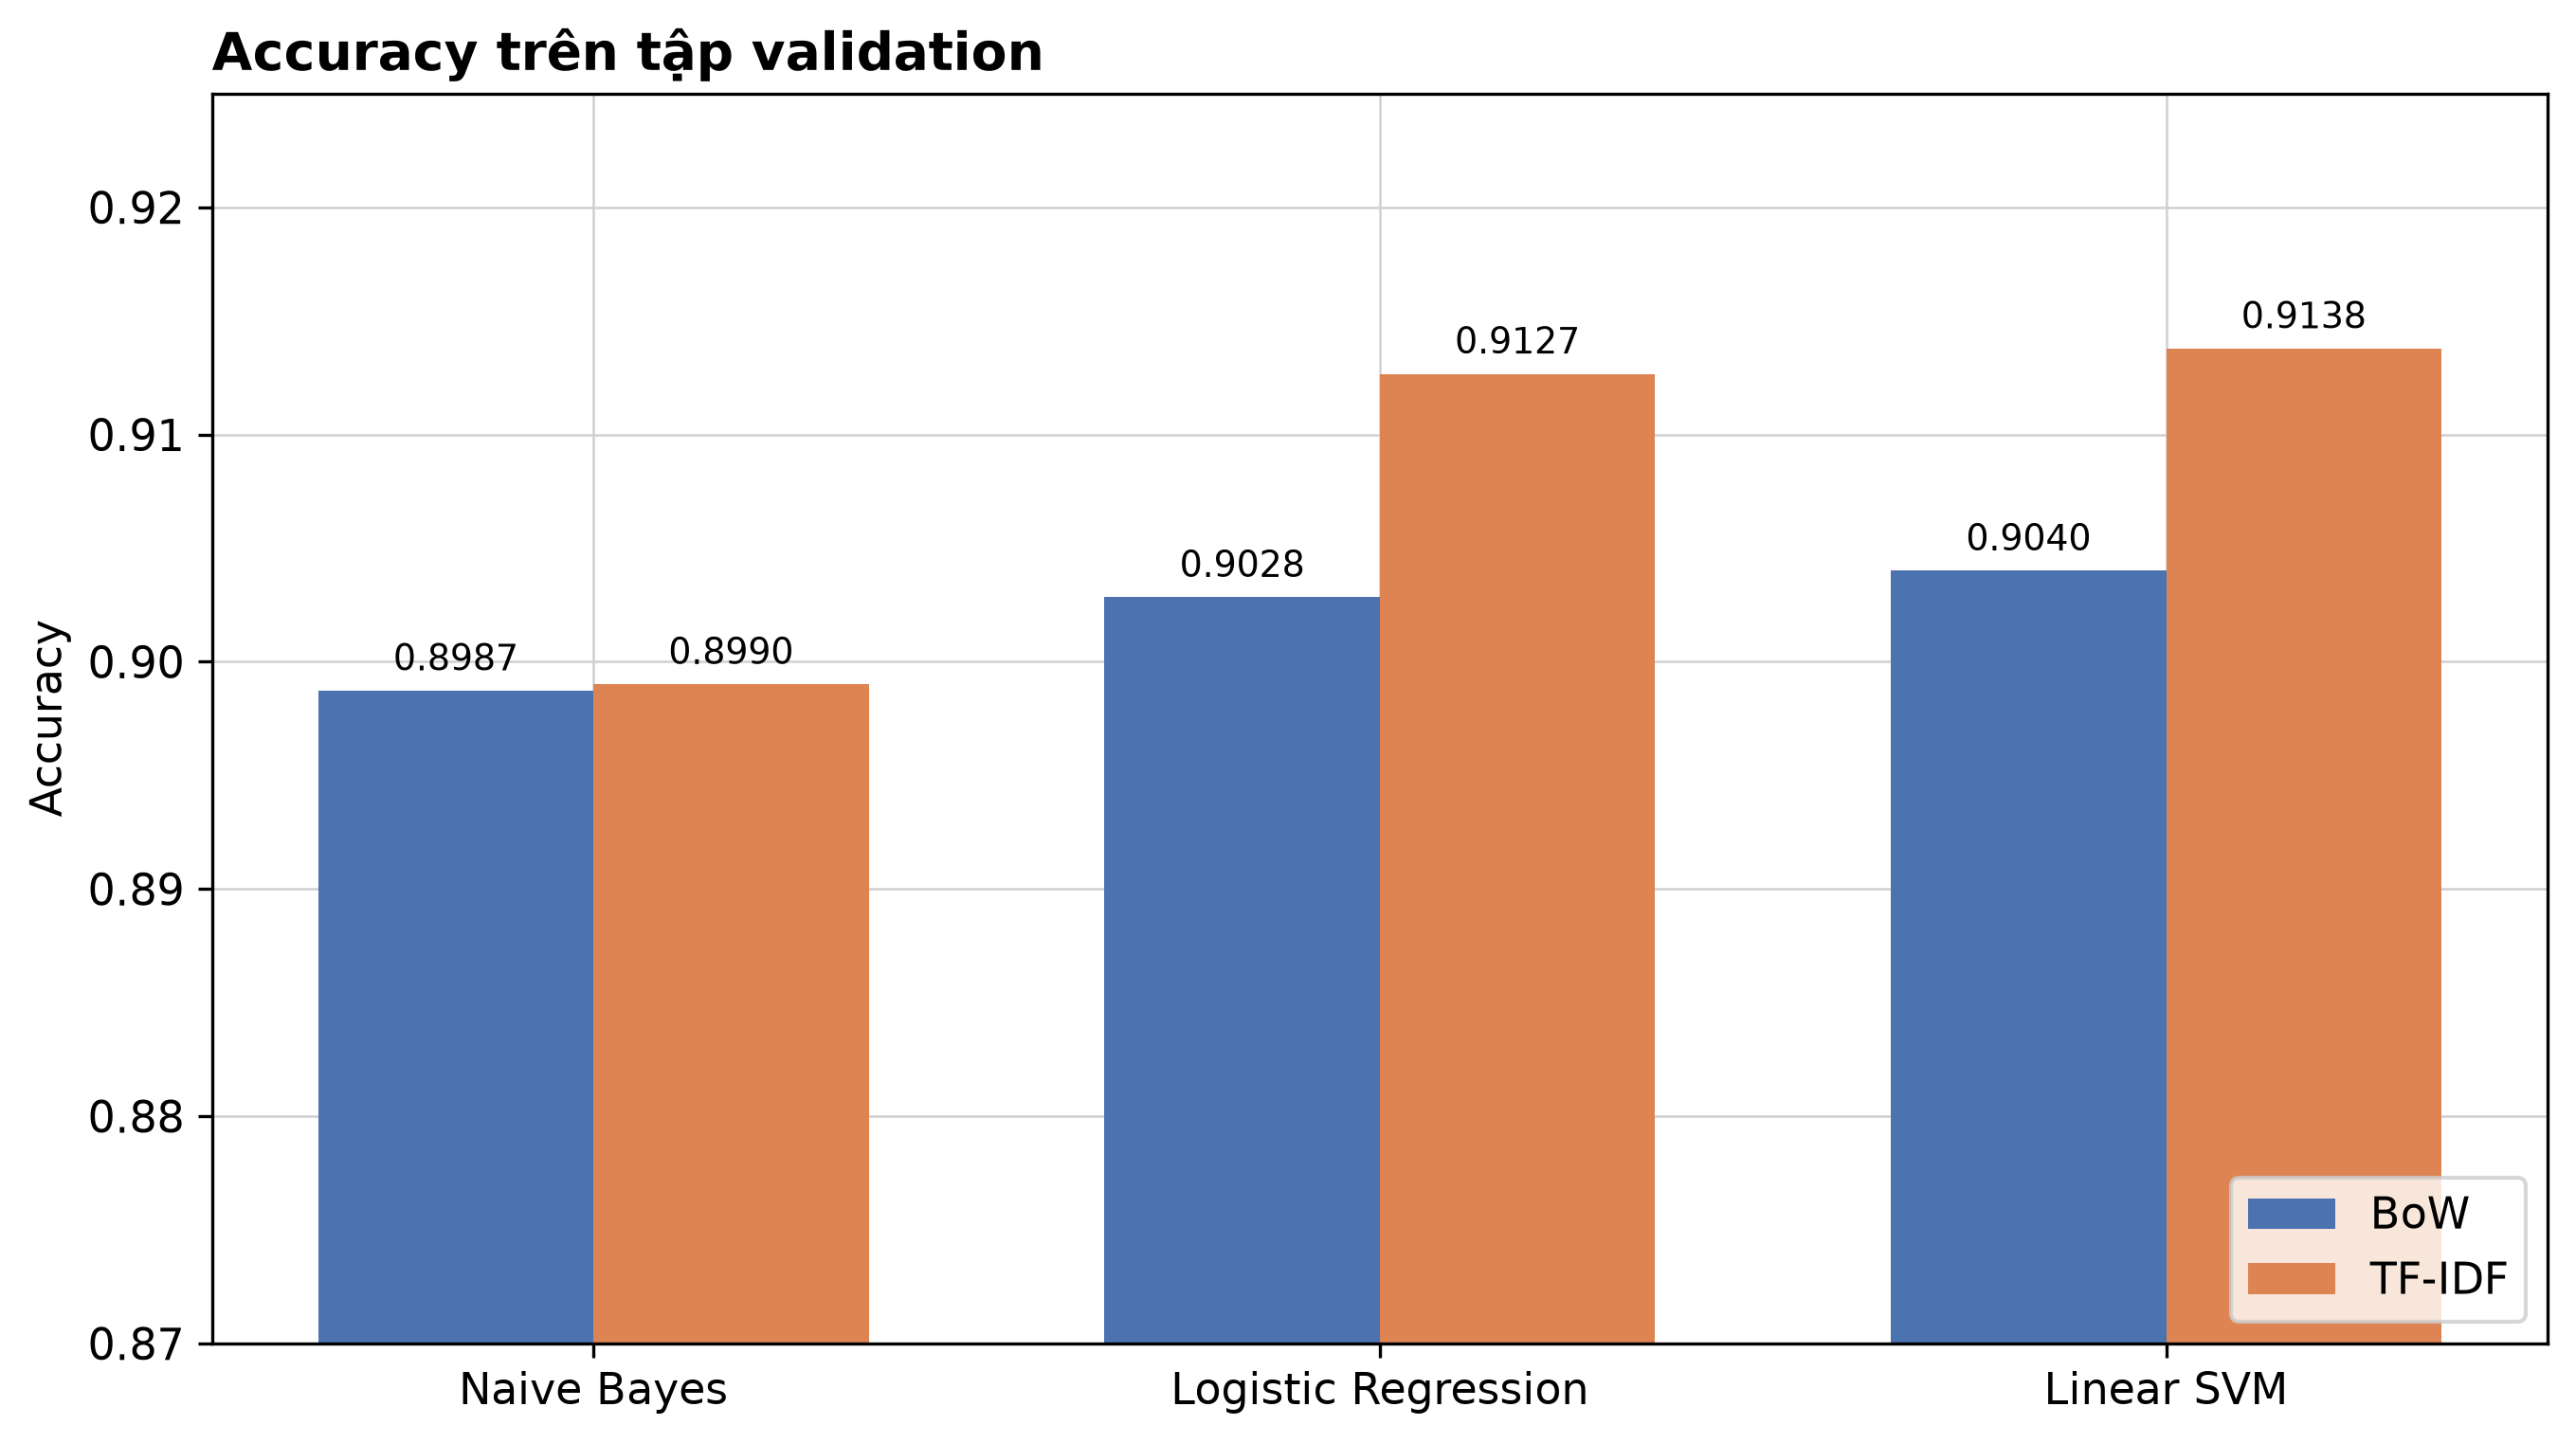
\includegraphics[width=0.92\textwidth,keepaspectratio]{graphics/model_accuracy_comparison.png}
  \caption{Accuracy của ba thuật toán trên BoW và TF--IDF (validation). Trục tung được thu hẹp quanh vùng $0{,}87$--$0{,}92$ để thấy chênh lệch giữa các cấu hình.}
  \label{fig:model-accuracy-comparison}
\end{figure}

\begin{figure}[H]
  \centering
  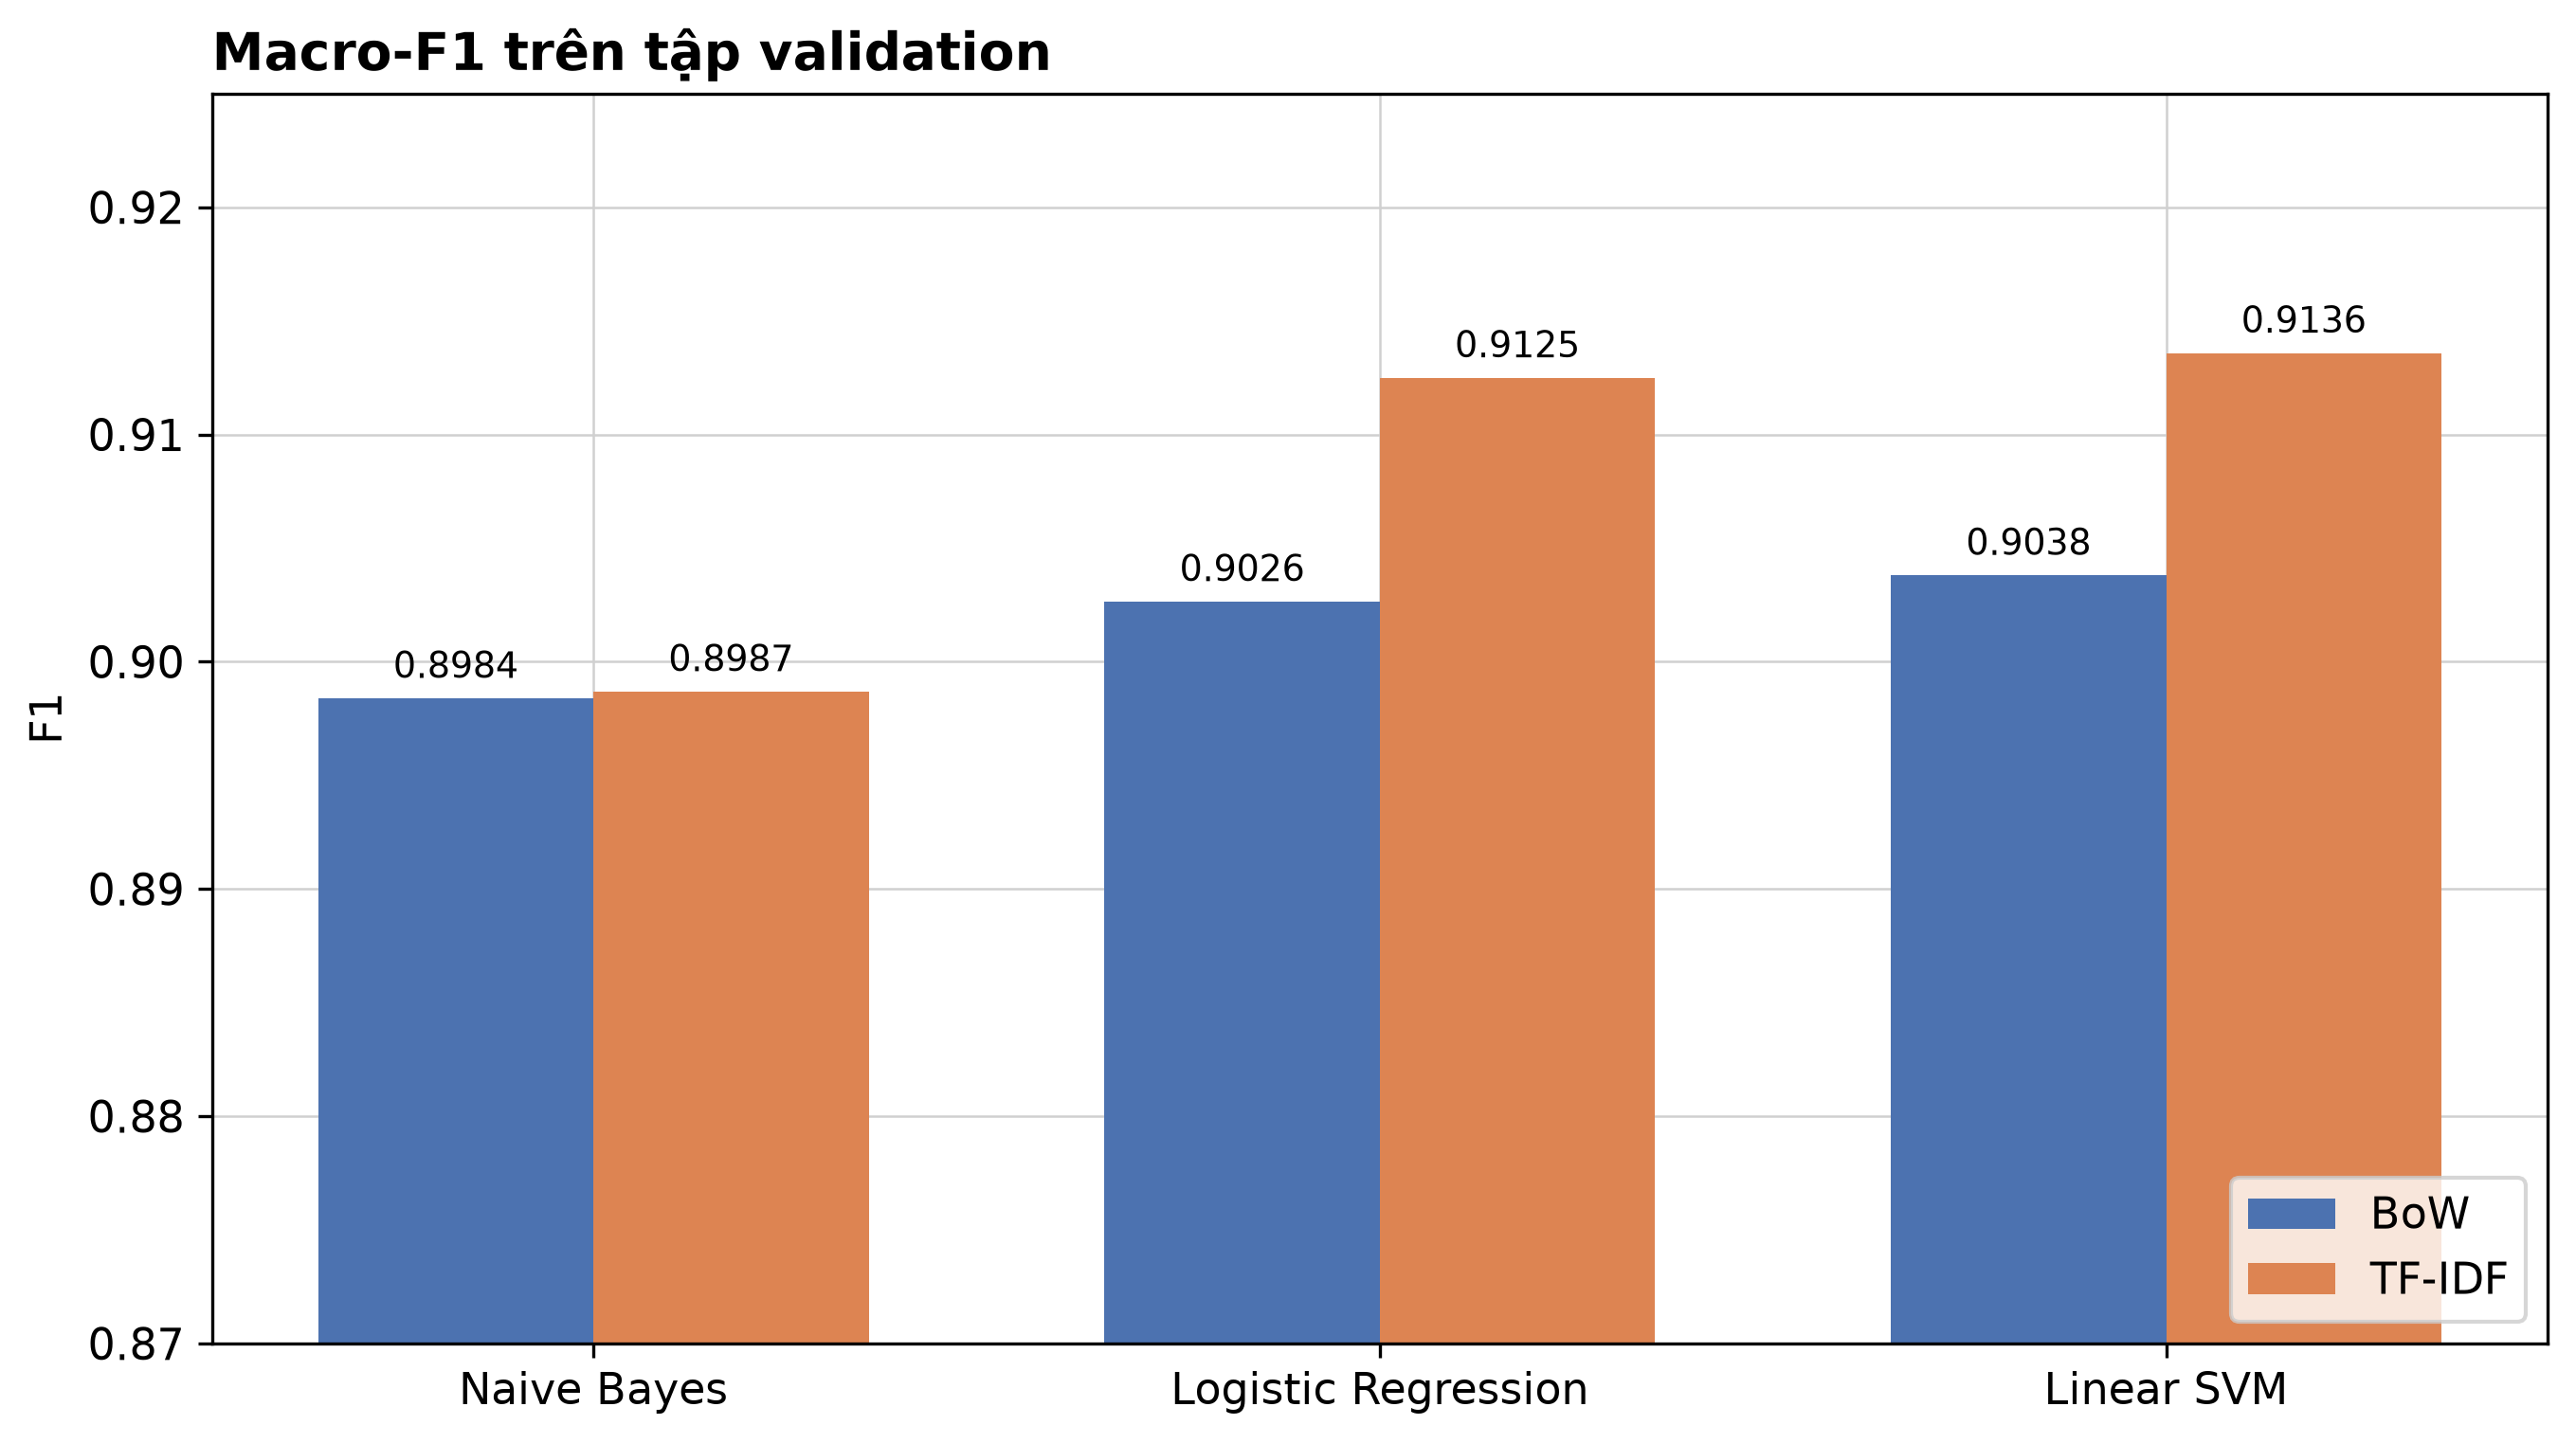
\includegraphics[width=0.92\textwidth,keepaspectratio]{graphics/model_f1_comparison.png}
  \caption{Macro-F1 của cùng sáu cấu hình trên tập validation. Thứ hạng gần như trùng với accuracy vì bốn lớp có cùng số mẫu.}
  \label{fig:model-f1-comparison}
\end{figure}

\begin{figure}[H]
  \centering
  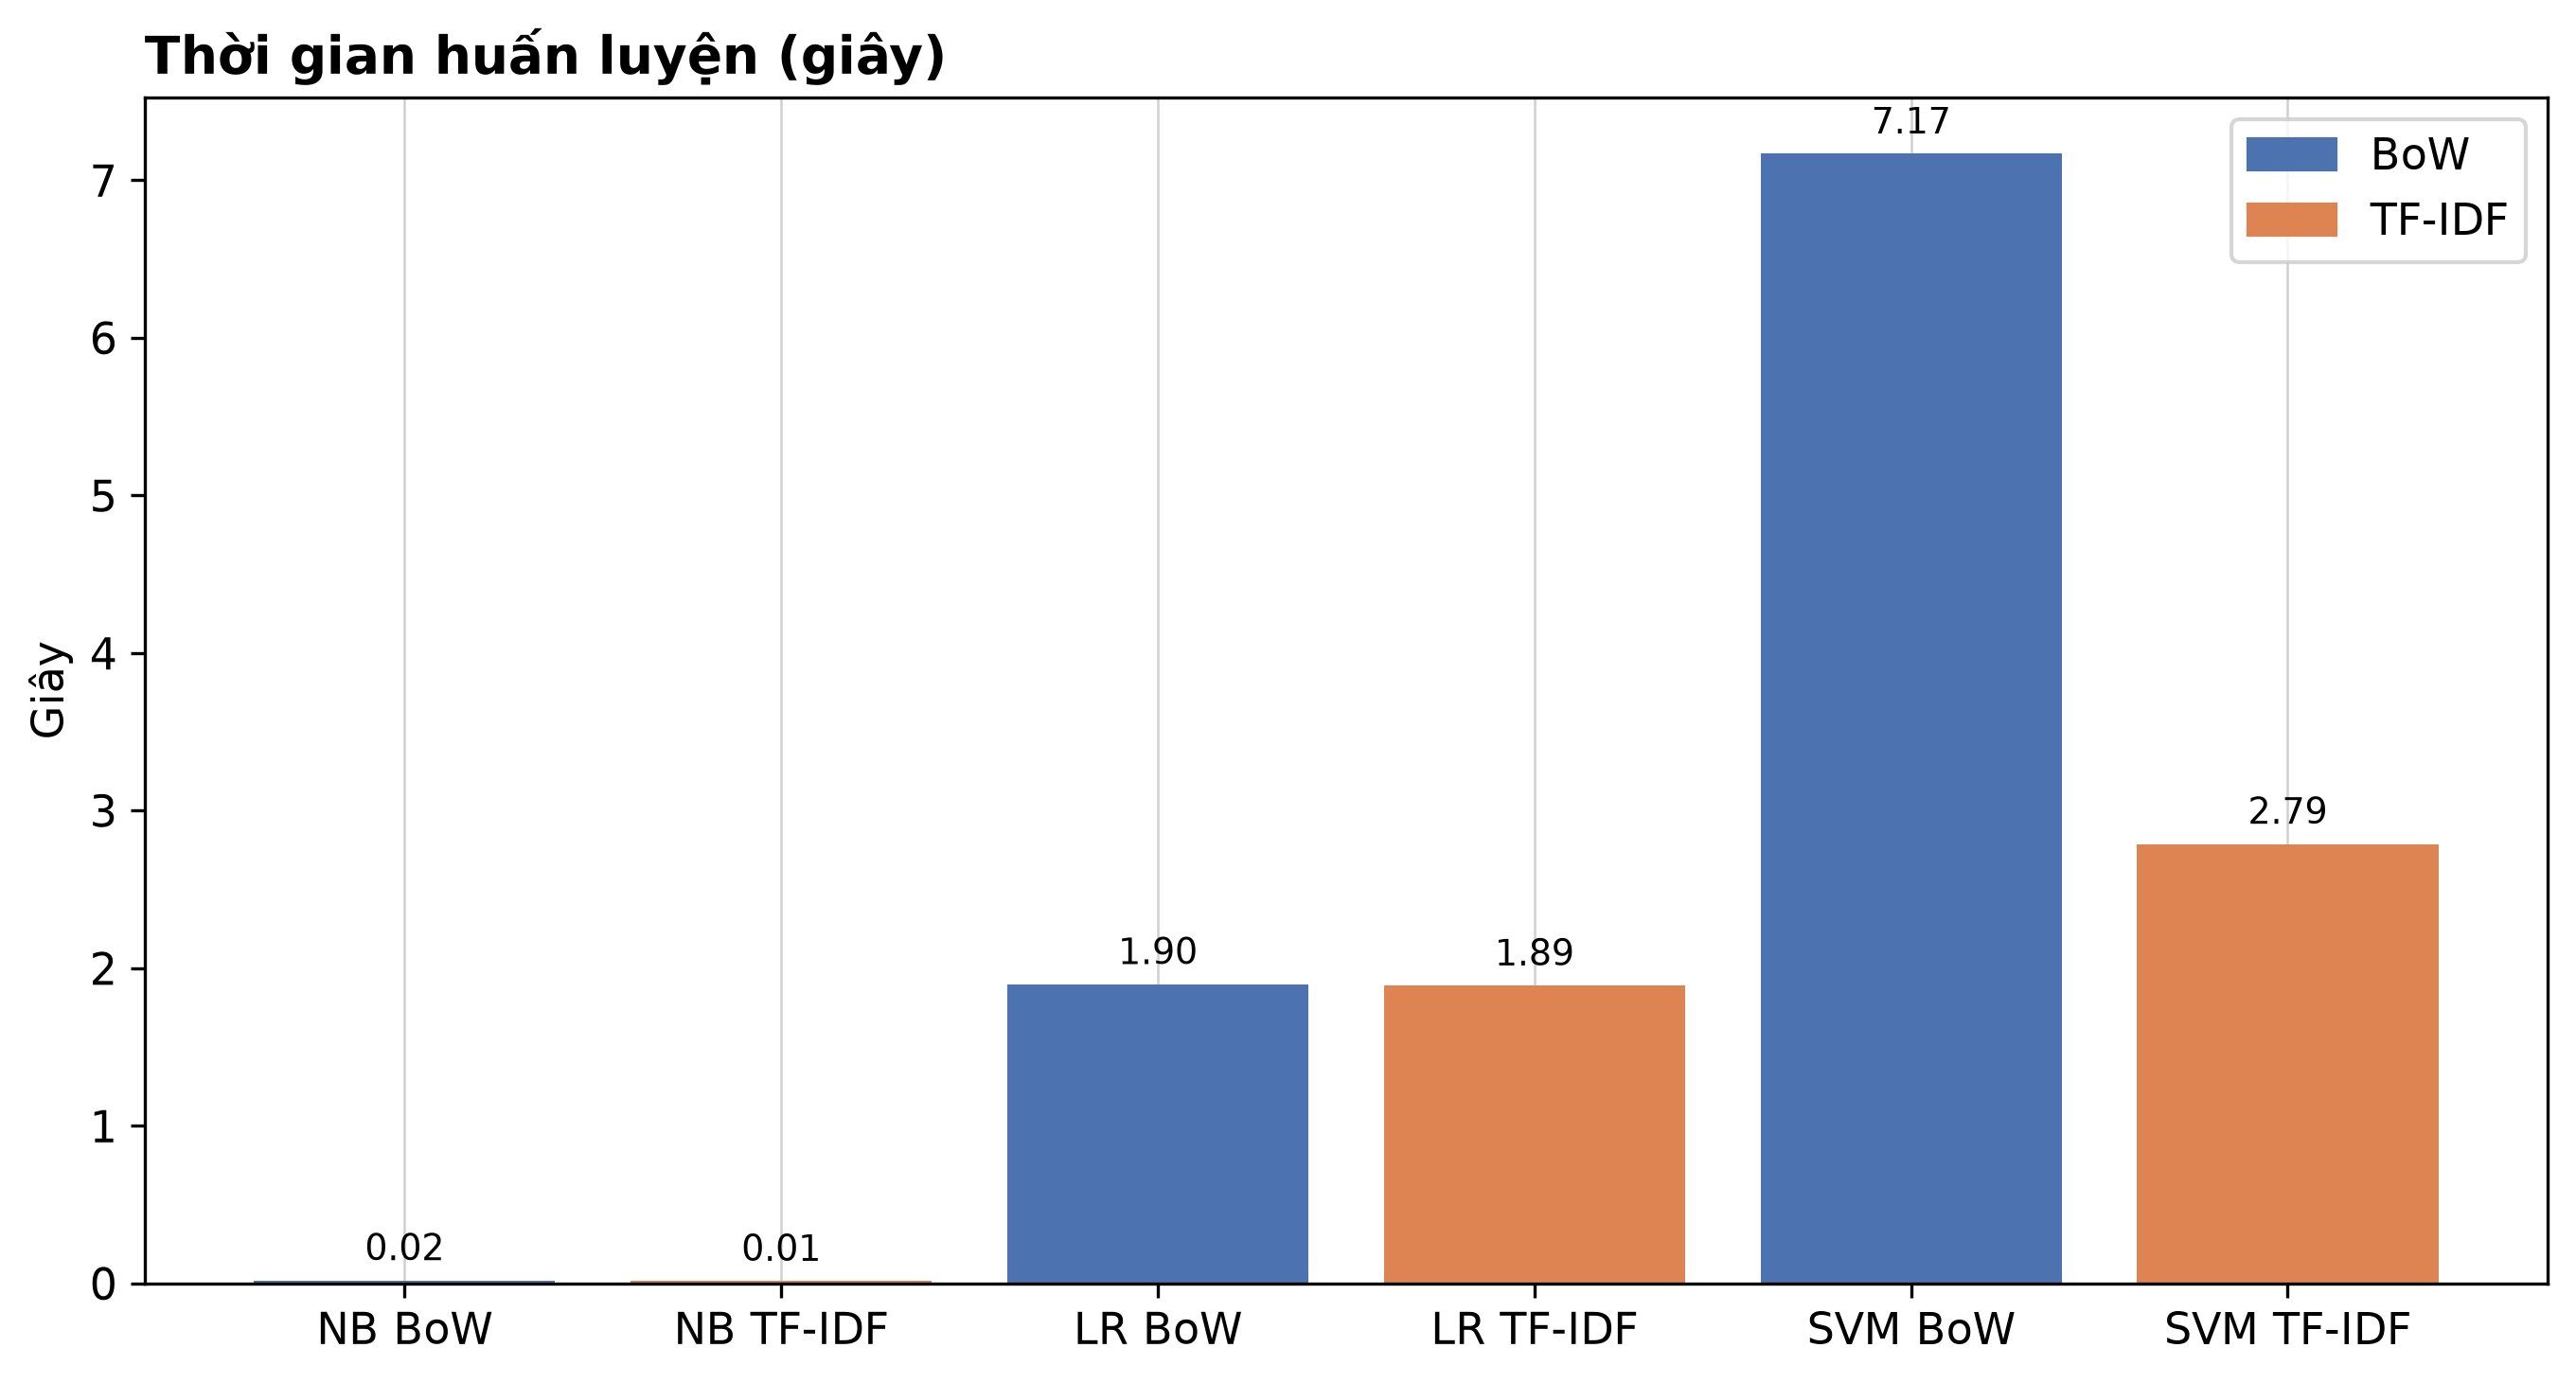
\includegraphics[width=0.92\textwidth,keepaspectratio]{graphics/training_time.png}
  \caption{Thời gian huấn luyện trên tập validation. Naive Bayes gần như tức thời. Linear SVM trên BoW là cấu hình chậm nhất; cùng thuật toán trên TF--IDF nhanh hơn rõ rệt.}
  \label{fig:training-time}
\end{figure}

\subsubsection{So sánh BoW và TF--IDF}

\firstparagraph Trung bình trên ba mô hình, BoW đạt accuracy \textbf{0,9018} và macro-F1 0,9016. TF--IDF đạt accuracy \textbf{0,9085} và macro-F1 0,9083. Như vậy, TF--IDF cao hơn khoảng \textbf{0,67} điểm phần trăm accuracy. Logistic Regression hưởng lợi nhiều nhất ($\mathbf{+0,99}$ điểm). Linear SVM tăng khoảng 0,98 điểm. Naive Bayes chỉ tăng rất nhẹ 0,03 điểm.

TF--IDF cũng giúp Linear SVM giảm thời gian huấn luyện từ \textbf{7,17} xuống \textbf{2,79} giây trong lần đo này. Kết quả thời gian phụ thuộc môi trường và phiên bản thư viện, nhưng hợp lý vì đặc trưng TF--IDF đã được scale và chuẩn hóa tốt hơn giá trị đếm thô.

\subsubsection{Thời gian và lỗi định tính}

\firstparagraph Hình~\ref{fig:training-time} cho thấy Naive Bayes chỉ cần khoảng \textbf{0,02} giây để huấn luyện, nên phù hợp làm đường cơ sở và kiểm thử pipeline. Logistic Regression cần khoảng hai giây. SVM--BoW là cấu hình chậm nhất. Ngược lại, SVM--TF--IDF vừa chính xác nhất vừa nhanh hơn đáng kể so với SVM--BoW. Chênh lệch khoảng \textbf{1,51} điểm accuracy giữa NB--BoW và mô hình tốt nhất tương ứng xấp xỉ \textbf{272} dự đoán đúng thêm trên 18.000 mẫu validation.

Lớp Sports có từ vựng riêng, trong khi Business và Sci/Tech chia sẻ nhiều từ về công ty và sản phẩm. Mức nhầm lẫn cụ thể được đo lại ở Mục~\ref{sec:error-analysis} trên cấu hình Linear SVM--TF--IDF khi đánh giá tập test.

Giới hạn chính của unigram là không mã hóa thứ tự từ và ngữ cảnh đa nghĩa. Đây cũng là hướng mở rộng đã nêu ở phần kết luận, dù pipeline tuyến tính đã đạt khoảng 91,4\% trên validation và 90,5\% trên test.

\subsection{Đánh giá tập test và phân tích lỗi theo lớp}
\label{sec:error-analysis}

\firstparagraph Bảng~\ref{tab:traditional-results} ghi nhận số liệu so sánh từ \texttt{results/comparison.csv} trên tập validation (được thực thi trong \texttt{notebooks/03\_model\_training.ipynb}). Sau khi xác định mô hình chiến thắng là Linear SVM kết hợp biểu diễn đặc trưng TF--IDF ($C=1{,}0$), nhóm tiến hành quy trình đánh giá độc lập trên toàn bộ 7.600 mẫu của tập kiểm tra thông qua \texttt{notebooks/04\_final\_test\_evaluation.ipynb}. Trên tập test độc lập, cấu hình này đạt accuracy $0{,}9051$ và macro-F1 $0{,}9049$. Mức sụt giảm hiệu năng so với tập validation chỉ khoảng $0{,}87$ điểm phần trăm. Độ chênh lệch tối thiểu này chứng minh mô hình có khả năng khái quát hóa vững chắc, hoàn toàn không bị rò rỉ thông tin (data leakage) hay quá khớp (overfitting) vào tập dữ liệu phát triển.

\begin{figure}[H]
  \centering
  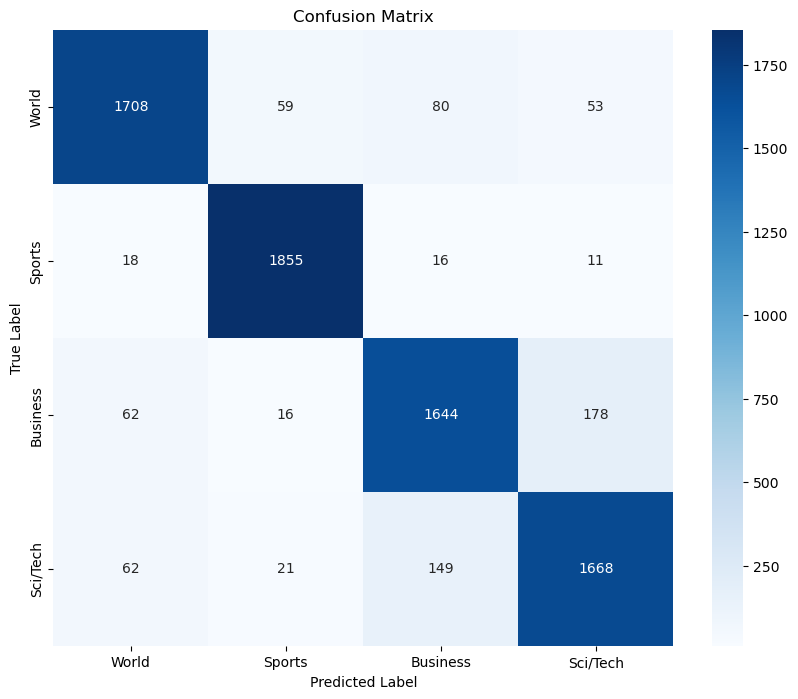
\includegraphics[width=0.72\textwidth,keepaspectratio]{graphics/confusion_matrix_svm_tfidf.png}
  \caption{Ma trận nhầm lẫn của Linear SVM + TF--IDF trên 7.600 mẫu test. Hàng là nhãn đúng, cột là nhãn dự đoán.}
  \label{fig:confusion-svm}
\end{figure}

\begin{table}[H]
  \centering
  \caption{Chỉ số theo lớp của Linear SVM + TF--IDF trên tập test}
  \label{tab:per-class}
  \small
  \renewcommand{\arraystretch}{1.15}
  \begin{tabular}{lrrrr}
    \toprule
    \textbf{Lớp} & \textbf{Precision} & \textbf{Recall} & \textbf{F1} & \textbf{Support} \\
    \midrule
    World    & 0,92 & 0,90 & 0,91 & 1.900 \\
    Sports   & 0,95 & 0,98 & \textbf{0,96} & 1.900 \\
    Business & 0,87 & 0,87 & \textbf{0,87} & 1.900 \\
    Sci/Tech & 0,87 & 0,88 & \textbf{0,88} & 1.900 \\
    \midrule
    Macro    & 0,9049 & 0,9051 & 0,9049 & 7.600 \\
    \bottomrule
  \end{tabular}
  \par\vspace{3pt}
  \parbox{0.86\textwidth}{\footnotesize\textit{Ghi chú:} Precision, recall và F1 từng lớp được làm tròn 2 chữ số theo classification report; hàng Macro giữ 4 chữ số từ các độ đo tổng hợp.}
\end{table}

\begin{figure}[H]
  \centering
  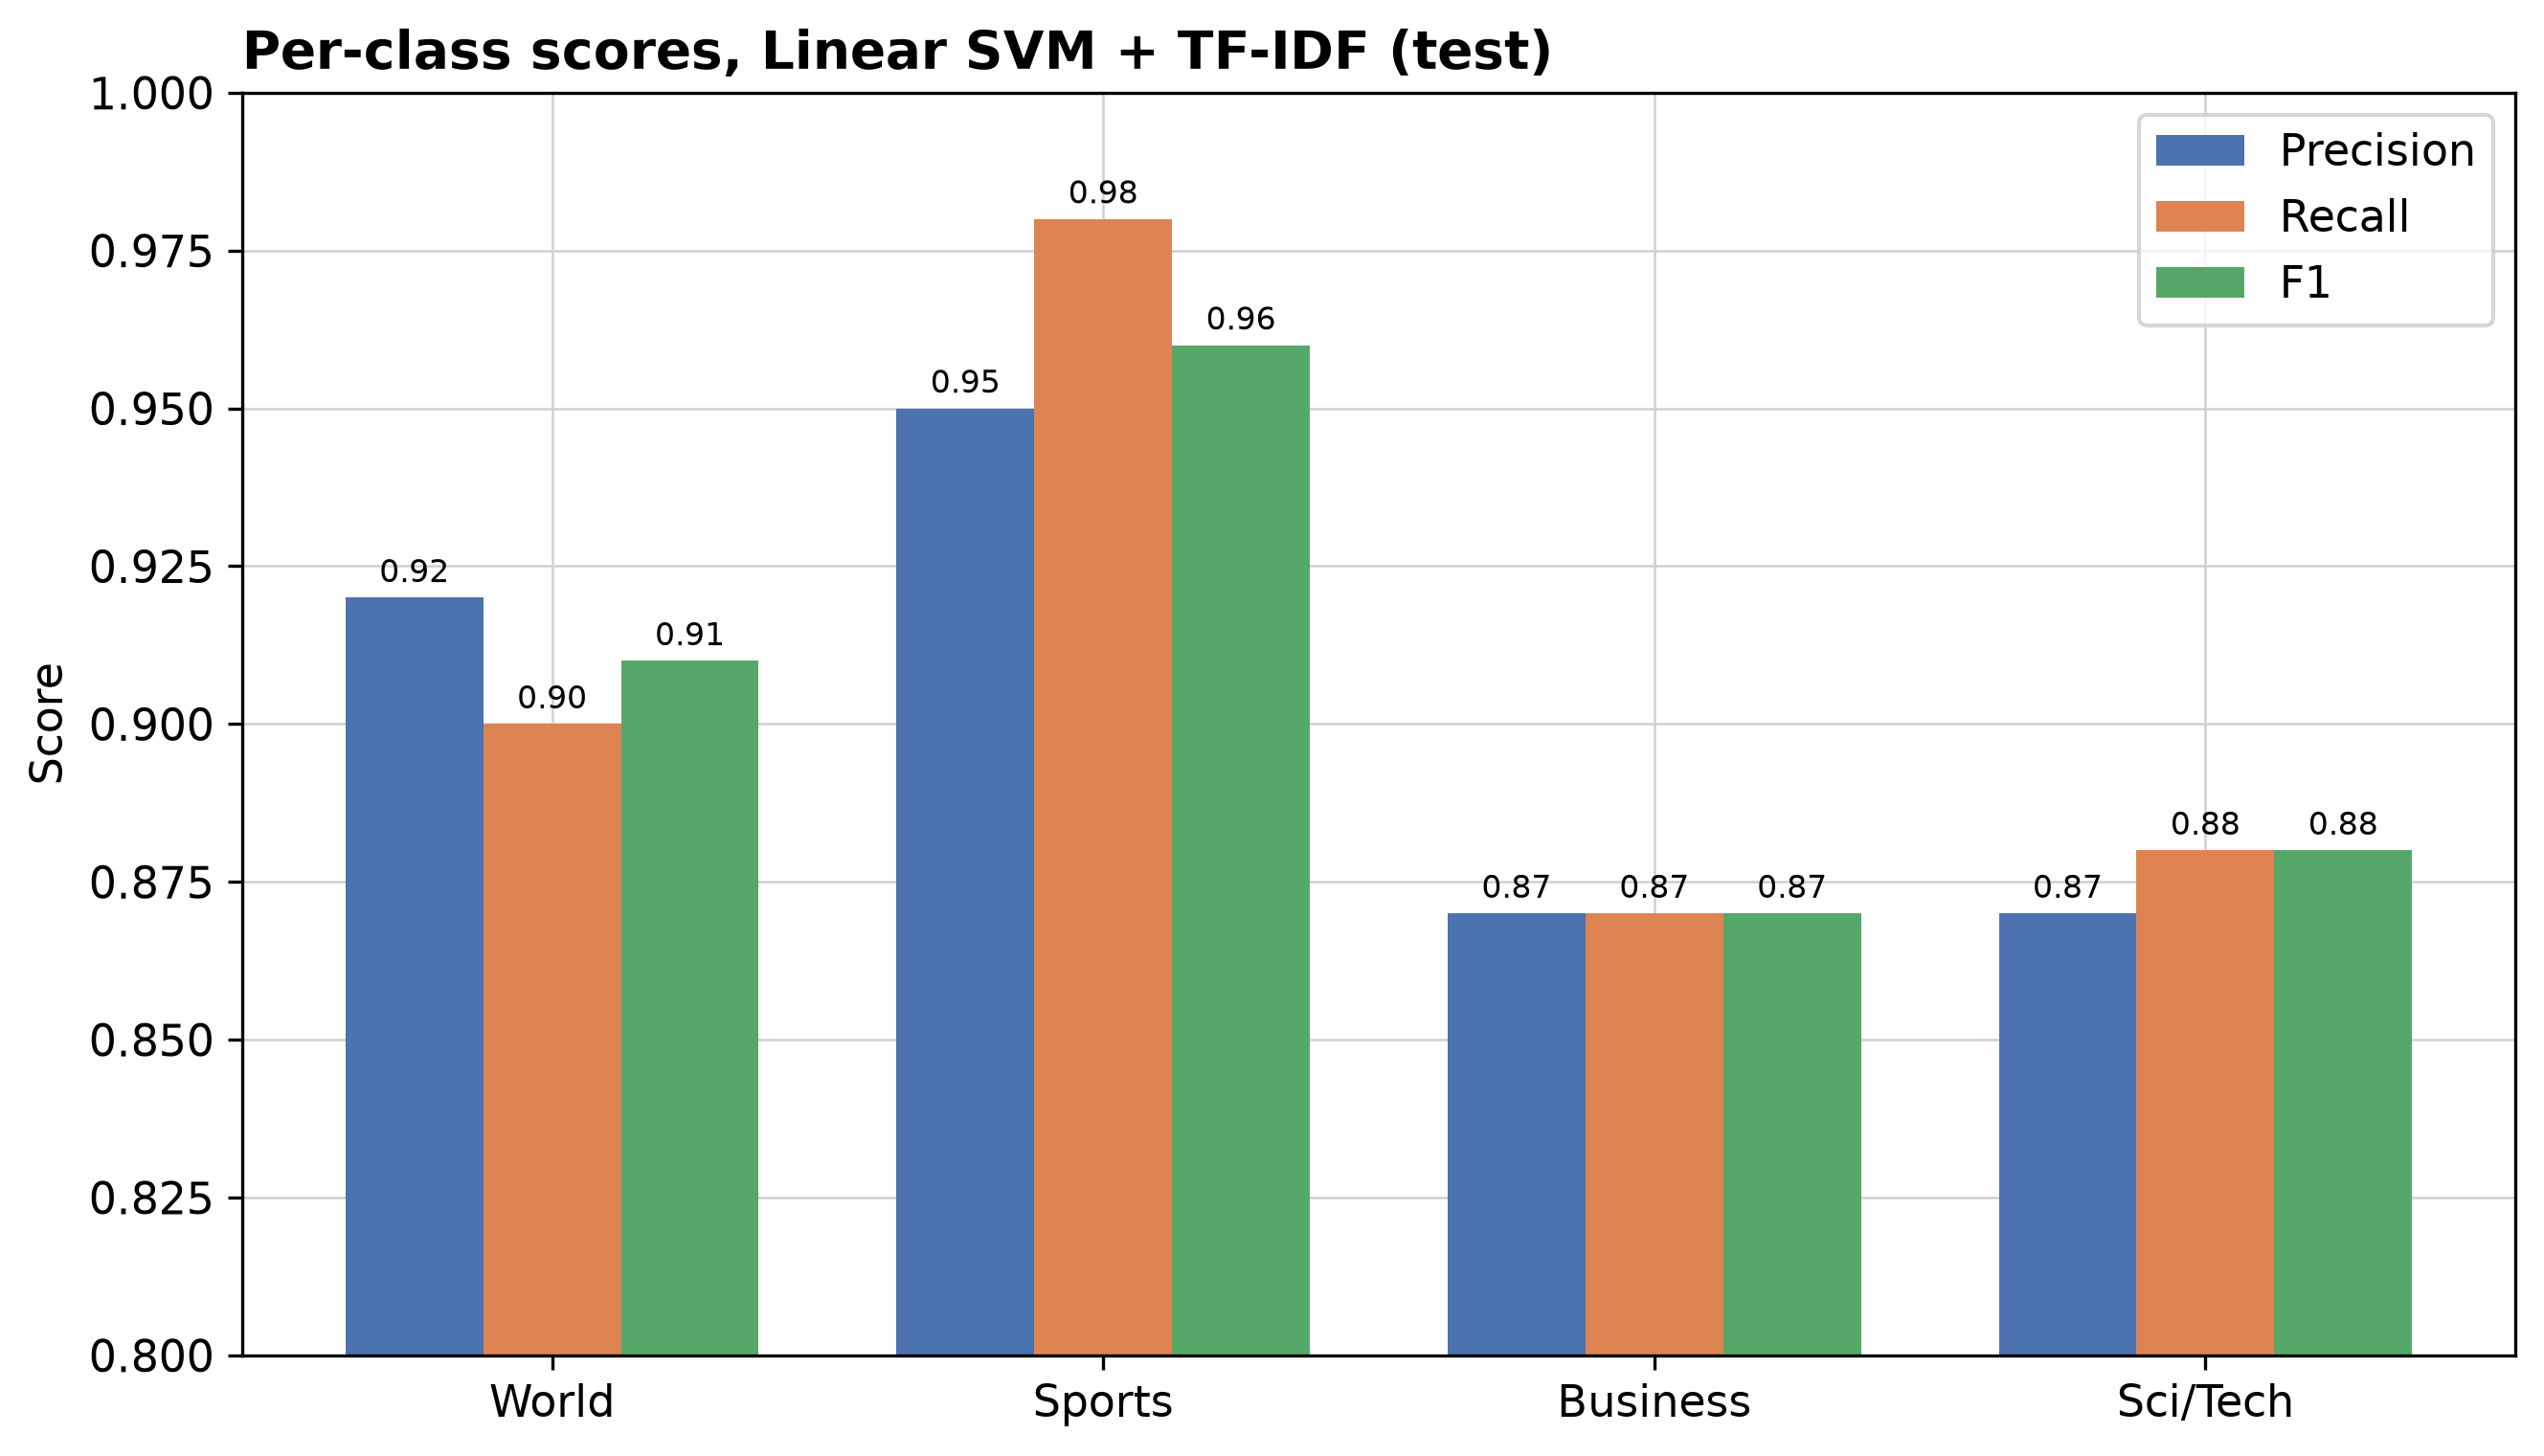
\includegraphics[width=0.82\textwidth,keepaspectratio]{graphics/per_class_f1.png}
  \caption{Precision, recall và F1 theo lớp trên tập test (Linear SVM + TF--IDF). Trục tung bắt đầu ở $0{,}80$ để thấy Sports tách khỏi hai lớp kinh doanh và công nghệ.}
  \label{fig:per-class}
\end{figure}

Lớp Sports đạt recall khoảng $0{,}98$ và F1 khoảng $0{,}96$. Lớp World cũng cao với F1 khoảng $0{,}91$. Hai lớp Business và Sci/Tech thấp hơn, với F1 lần lượt khoảng $0{,}87$ và $0{,}88$. Ma trận nhầm lẫn cho thấy lỗi tập trung chủ yếu ở cặp Business--Sci/Tech. Vì vậy, accuracy khoảng $0{,}91$ không có nghĩa bốn lớp cùng khó. Phần khó chủ yếu nằm ở ranh giới giữa tin kinh doanh và tin công nghệ.

Ba mẫu sau minh họa ranh giới đó và không phải là lỗi ngẫu nhiên:

\begin{reportitems}
  \item Nhãn thật là Sci/Tech, mô hình dự đoán Business: \textit{IBM to hire even more new workers... biggest headcount since 1991.} Nội dung nói về tuyển dụng của một hãng máy tính.
  \item Nhãn thật là Sci/Tech, mô hình dự đoán Business: \textit{Dell exits low-end China consumer PC market.} Nội dung vừa liên quan sản phẩm công nghệ, vừa liên quan quyết định thị trường.
  \item Nhãn thật là Business, mô hình dự đoán Sci/Tech: \textit{Intel to delay product aimed for high-definition TVs.} Nội dung nói về việc hãng bán dẫn lùi lịch ra mắt một con chip.
\end{reportitems}

Các hệ số dương lớn nhất của SVM cho thấy mô hình học được từ đúng chủ đề, nhưng đồng thời cũng bị kéo bởi nhiễu thu thập dữ liệu. Lớp Sports gắn với \textit{nascar}, \textit{nba}, \textit{coach}, \textit{ncaa}. Lớp World gắn với \textit{iraqi}, \textit{palestinian}, \textit{darfur}, \textit{afghan}, nhưng cũng xuất hiện \textit{afp} và một token dính từ thẻ HTML. Lớp Business có \textit{investing} cạnh \textit{hellip} và \textit{href}. Lớp Sci/Tech có \textit{nasa}, \textit{xbox}, \textit{wifi} cạnh các mảnh XML như \textit{qtypesym}. Vì SVM tuyến tính cộng trọng số từng từ, việc làm sạch thực thể HTML trước bước lọc ký tự là cải tiến tiền xử lý có căn cứ, chứ không chỉ dựa trên cảm tính.

\begin{figure}[H]
  \centering
  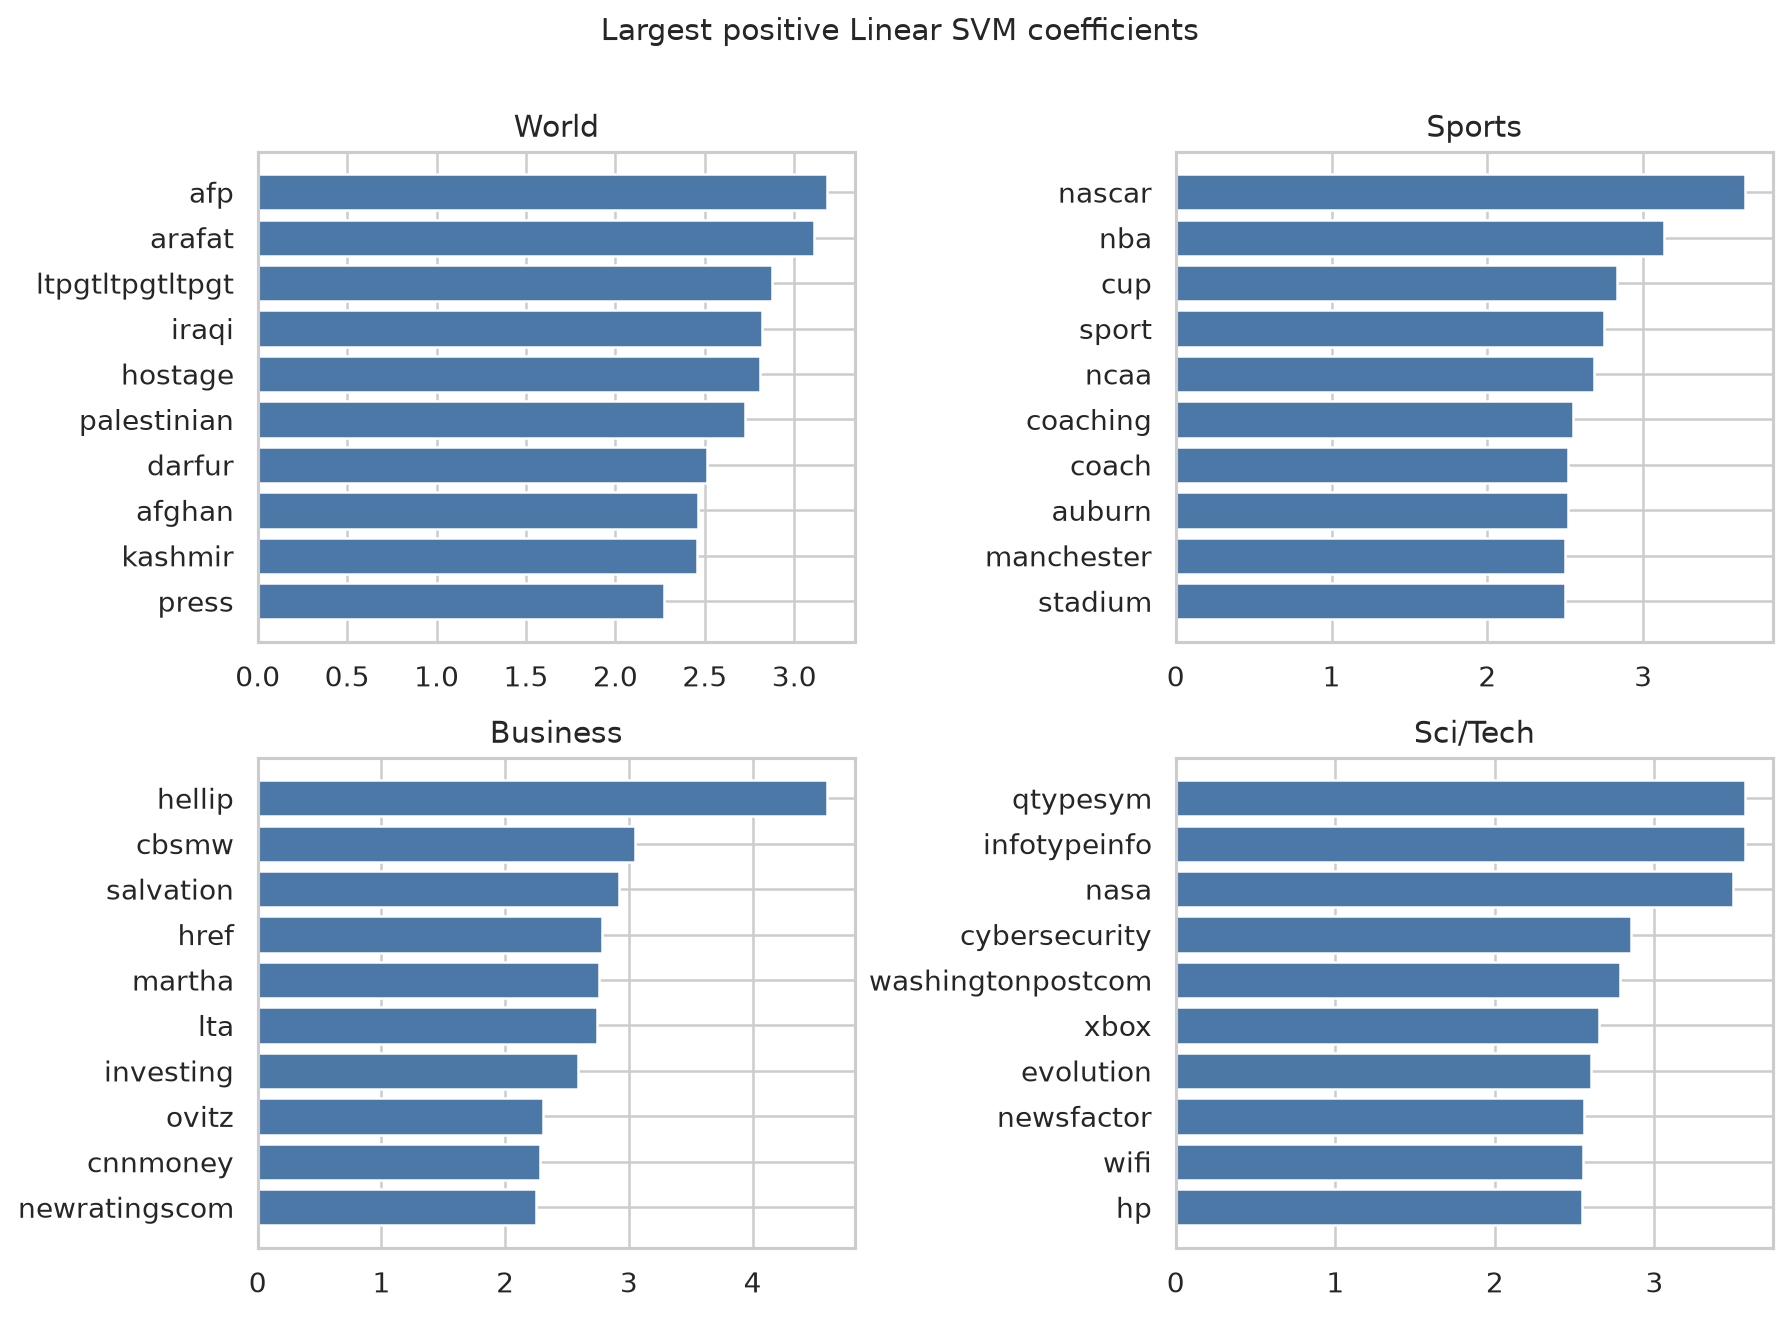
\includegraphics[width=0.92\textwidth,keepaspectratio]{graphics/svm_top_coefficients.png}
  \caption{Mười hệ số dương lớn nhất của Linear SVM trên từng lớp. Trục hoành là trọng số trong không gian TF--IDF.}
  \label{fig:svm-coef}
\end{figure}

\subsection{Thực nghiệm lựa chọn đặc trưng (Feature Selection)}

\firstparagraph Để khảo sát xem việc giảm số chiều có giúp loại bỏ nhiễu và tăng tốc độ mô hình mà không làm giảm độ chính xác hay không, nhóm đã triển khai module \texttt{experiments/\allowbreak feature\_selection.py} với ba phương pháp chọn thuộc tính:
\begin{enumerate}[leftmargin=2em,itemsep=5pt]
  \item \textbf{Kiểm định Chi-bình phương ($\chi^2$):} Đánh giá mức độ phụ thuộc thống kê giữa sự xuất hiện của từ $t$ và từng lớp chủ đề $k$:
  \begin{equation}
    \chi^2(t, k) = \frac{N (AD - BC)^2}{(A+B)(C+D)(A+C)(B+D)},
    \label{eq:chi2}
  \end{equation}
  trong đó $A$ là số văn bản lớp $k$ chứa $t$; $B$ là số văn bản ngoài lớp $k$ chứa $t$; $C$ là số văn bản lớp $k$ không chứa $t$; $D$ là số văn bản ngoài lớp $k$ không chứa $t$; và $N=A+B+C+D$. Điểm đặc trưng tổng hợp là $\chi^2_{\max}(t) = \max_k \chi^2(t, k)$.
  \item \textbf{Thông tin tương hỗ (Mutual Information):} Đo lượng thông tin thu được về nhãn chủ đề khi biết sự hiện diện của từ $t$:
  \begin{equation}
    I(t; Y) = \sum_{t \in \{0, 1\}} \sum_{k=1}^K P(t, Y=k) \log_2 \frac{P(t, Y=k)}{P(t) P(Y=k)}.
    \label{eq:mutual-info}
  \end{equation}
  \item \textbf{Mô hình cây (Tree-based):} Sử dụng kỹ thuật \texttt{SelectFromModel} kết hợp ensemble \texttt{RandomForest} đo lường mức giảm độ tạp chất Gini (Mean Decrease Impurity) để xếp hạng các đặc trưng quan trọng nhất.
\end{enumerate}

Thực nghiệm trên phương pháp Chi-bình phương được tiến hành bằng cách giữ lại top $k$ từ phân biệt nhất từ không gian TF--IDF ban đầu, sau đó huấn luyện mô hình Linear SVM ($C=1{,}0$). Bảng~\ref{tab:chi2} và Hình~\ref{fig:chi2} trình bày kết quả khi quét $k \in \{500, 1000, 2000, 5000\}$.

\begin{table}[H]
  \centering
  \caption{Hiệu năng Linear SVM sau khi chọn đặc trưng bằng Chi-bình phương}
  \label{tab:chi2}
  \small
  \renewcommand{\arraystretch}{1.12}
  \begin{tabular}{rrrr}
    \toprule
    \textbf{Số đặc trưng ($k$)} & \textbf{Accuracy} & \textbf{Macro-F1} & \textbf{Train (s)} \\
    \midrule
    500   & 0,8628 & 0,8620 & 1,47 \\
    1.000 & 0,8854 & 0,8850 & 1,71 \\
    2.000 & 0,9021 & 0,9018 & 2,04 \\
    5.000 & \textbf{0,9138} & \textbf{0,9136} & 2,82 \\
    \bottomrule
  \end{tabular}
  \par\vspace{3pt}
  \parbox{0.86\textwidth}{\footnotesize\textit{Ghi chú:} Điểm số tăng đơn điệu theo $k$. Số liệu lấy từ thực nghiệm trong \texttt{experiments/\allowbreak feature\_selection.py}.}
\end{table}

\begin{figure}[H]
  \centering
  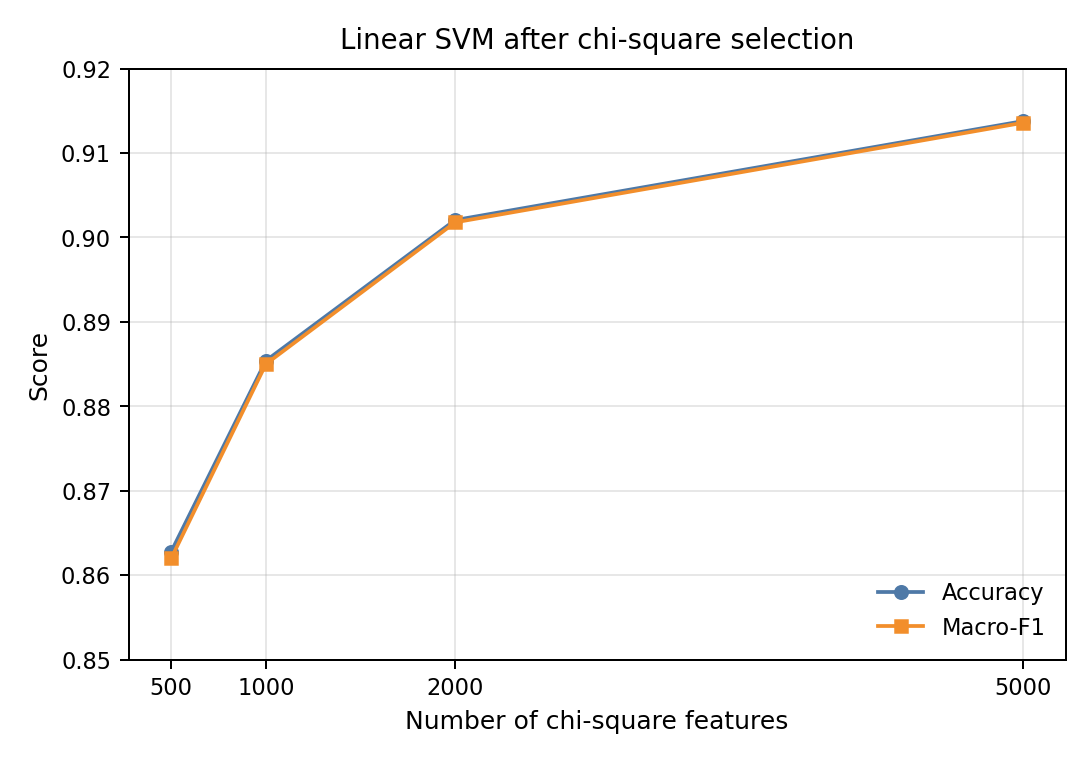
\includegraphics[width=0.78\textwidth,keepaspectratio]{graphics/chi2_feature_selection.png}
  \caption{Accuracy và macro-F1 tăng khi giữ nhiều đặc trưng chi-bình phương hơn. Tại $k=500$, cả hai độ đo còn khoảng $0{,}86$.}
  \label{fig:chi2}
\end{figure}

Kết quả chứng minh rằng với bài toán phân loại tin tức đa lớp AG News, không gian 5.000 từ vựng ban đầu chưa bị hiện tượng bão hòa hay quá nhiều chiều dẫn đến quá khớp. Khi cắt giảm $k$ xuống dưới 2.000 từ (đặc biệt tại $k=500$, accuracy sụt giảm xuống $0{,}8628$), hiệu năng mô hình giảm sút rõ rệt do việc lược bỏ quá mức đã tước đi các từ khóa chuyên biệt theo từng chủ đề hẹp (như tên riêng địa chính trị, tên vận động viên, hoặc thuật ngữ công nghệ mới nổi). Do đó, cấu hình giữ nguyên 5.000 đặc trưng mang lại sự cân bằng tối ưu nhất giữa độ chính xác và chi phí bộ nhớ.

\section{Tổ chức và quản lý mã nguồn của nhóm}

\firstparagraph Nhóm quản lý mã nguồn bằng Git tại \url{https://github.com/Vhoamochii/ML_assignment}. Logic dùng chung được đặt trong \texttt{src/}. Quy trình thí nghiệm nằm trong \texttt{notebooks/}. Các tinh chỉnh bổ sung nằm trong \texttt{experiments/}. Seed \texttt{random\_state=42} được cố định để tái lập kết quả. Dữ liệu thô, ma trận đặc trưng và mô hình lớn không được commit vào kho mã. Liên kết tải nằm trong README và \texttt{models/model\_links.txt}.

\subsection{Cấu trúc thư mục}

\begin{lstlisting}[
  language={},
  basicstyle=\ttfamily\footnotesize\color{black},
  numbers=none,
  frame=single,
  backgroundcolor=\color{gray!6},
  rulecolor=\color{gray!45},
  xleftmargin=0.025\textwidth,
  xrightmargin=0.025\textwidth,
  framexleftmargin=8pt,
  framexrightmargin=8pt,
  framextopmargin=6pt,
  framexbottommargin=6pt,
  columns=fullflexible,
  keepspaces=true,
  showstringspaces=false
]
ML_assignment/
|-- data/
|   |-- raw/                           # Du lieu goc: train.csv (120k), test.csv (7.6k)
|   `-- processed/                     # Du lieu da tien xu ly va ma tran dac trung
|-- notebooks/                         # 4 Notebooks theo luong pipeline tuan tu
|   |-- 01_data_analysis.ipynb         # Phan tich va kham pha dac trung du lieu (EDA)
|   |-- 02_preprocessing.ipynb         # Lam sach van ban, trich xuat dac trung BoW & TF-IDF
|   |-- 03_model_training.ipynb        # Huan luyen 6 to hop mo hinh tren tap validation
|   `-- 04_final_test_evaluation.ipynb # Danh gia mo hinh tot nhat tren tap test doc lap
|-- src/                               # Ma nguon module hoa (Modular Architecture)
|   |-- data_loader.py                 # Nap va phan chia tap du lieu
|   |-- preprocessing.py               # Tien xu ly van ban, tokenization, lemmatization
|   |-- evaluation.py                  # Tinh toan metrics va ve bieu do confusion matrix
|   |-- utils.py                       # Luu tru / nap mo hinh (.pkl) va tien ich
|   `-- models/                        # Dinh nghia cac thuat toan Machine Learning
|       |-- baseline.py                # Dummy classifier, Naive Bayes, Logistic Regression
|       `-- traditional_ml.py          # Linear SVM, SVC, Random Forest, Decision Tree
|-- experiments/                       # Thi nghiem lua chon dac trung
|   `-- feature_selection.py           # Lua chon dac trung (Chi2, Mutual Info, Tree-based)
|-- models/
|   `-- model_links.txt                # Lien ket luu tru cac mo hinh lon
|-- results/
|   |-- comparison.csv                 # Bang tong hop ket qua tren tap validation
|   `-- figures/                       # Cac bieu do truc quan hoa va ma tran nham lan
|-- Dockerfile                         # Thiet lap moi truong Docker dong nhat
|-- requirements.txt                   # Danh sach goi phu thuoc Python
|-- README.md                          # Huong dan van hanh va tai lap ket qua
`-- .gitignore
\end{lstlisting}

\subsection{Luồng chạy tái lập}

\firstparagraph Quy trình tái lập kết quả thực nghiệm được chuẩn hóa qua hai phương thức triển khai môi trường và một chuỗi thực thi tuần tự khép kín:

\begin{enumerate}[leftmargin=2em,itemsep=5pt]
  \item \textbf{Khởi tạo môi trường:} 
  \begin{itemize}[leftmargin=1.5em,itemsep=2pt]
    \item \textit{Phương thức 1 (Docker):} Xây dựng image và khởi chạy container với cổng 8888:
    \par\vspace{2pt}
    \texttt{docker build -t ag-news-ml-project .}
    \par\vspace{2pt}
    \texttt{docker run -p 8888:8888 -v \$\{PWD\}:/app\allowbreak{} ag-news-ml-project}
    \item \textit{Phương thức 2 (Local pip):} Cài đặt các gói phụ thuộc qua \texttt{pip install -r requirements.txt} và tải từ điển NLTK (\texttt{punkt}, \texttt{stopwords}, \texttt{wordnet}).
  \end{itemize}
  \item \textbf{Chuẩn bị dữ liệu:} Tải bộ dữ liệu AG News từ Kaggle và đặt hai tệp \texttt{train.csv} (120.000 mẫu) và \texttt{test.csv} (7.600 mẫu) vào thư mục \texttt{data/raw/}.
  \item \textbf{Khám phá dữ liệu (EDA):} Mở và thực thi \texttt{notebooks/\allowbreak 01\_data\_analysis.ipynb} để thống kê phân phối lớp, độ dài văn bản và xuất biểu đồ vào \texttt{results/\allowbreak figures/}.
  \item \textbf{Tiền xử lý và tạo đặc trưng:} Thực thi \texttt{notebooks/\allowbreak 02\_preprocessing.ipynb} để làm sạch văn bản, tách tập train/validation (102.000 / 18.000 mẫu), khớp vectorizer và lưu ma trận BoW, TF--IDF vào \texttt{data/\allowbreak processed/}.
  \item \textbf{Huấn luyện mô hình:} Thực thi \texttt{notebooks/\allowbreak 03\_model\_training.ipynb} để huấn luyện sáu tổ hợp mô hình, đánh giá trên 18.000 mẫu validation, lưu mô hình vào \texttt{models/} và ghi bảng \texttt{results/\allowbreak comparison.csv}.
  \item \textbf{Đánh giá kiểm thử độc lập:} Thực thi \texttt{notebooks/\allowbreak 04\_final\_\allowbreak test\_\allowbreak evaluation\allowbreak .ipynb} để nạp mô hình tối ưu (\texttt{linear\_svm\_tfidf.pkl}), dự đoán một lần trên 7.600 mẫu test, vẽ ma trận nhầm lẫn và báo cáo theo lớp.
  \item \textbf{Thực thi thí nghiệm mở rộng:} Chạy từ terminal tập lệnh \texttt{python experiments/\allowbreak feature\_selection.py} để khảo sát ảnh hưởng của việc lựa chọn đặc trưng với Chi-bình phương, Mutual Information và Tree-based.
\end{enumerate}

Thứ tự thực thi từ notebook 01 đến 04 cần được tuân thủ nghiêm ngặt, vì đầu ra của giai đoạn trước đóng vai trò dữ liệu đầu vào cho giai đoạn kế tiếp. Toàn bộ quá trình sử dụng chung một seed ngẫu nhiên \texttt{random\_state=42} nhằm bảo đảm tính tiền định (determinism) và tính tái lập hoàn toàn ($100\%$ reproducibility).

\section{Thảo luận}

\firstparagraph AG News phù hợp với bài toán phân loại văn bản vì bộ dữ liệu đã có nhãn sẵn, có tập kiểm tra tách biệt, bốn lớp cân bằng và độ dài văn bản vừa đủ để BoW cùng TF--IDF chạy được trên CPU. Khó khăn chính \textbf{không nằm ở mất cân bằng lớp}, mà nằm ở nhiễu từ quá trình thu thập dữ liệu, ở từ đa nghĩa, và ở sự chồng lấn từ vựng giữa Business với Sci/Tech khi cùng nói về công ty hay sản phẩm. Ma trận nhầm lẫn trên tập test củng cố nhận định này: \textbf{lớp Sports gần như được phân tách rõ}, trong khi lỗi còn lại tập trung chủ yếu ở cặp Business--Sci/Tech.

Vì mỗi lớp chiếm đúng 25\%, accuracy là độ đo hợp lệ. Một lớp không thể làm tăng điểm chung chỉ nhờ có nhiều mẫu hơn. Báo cáo vẫn dùng thêm macro-F1 để kiểm tra xem có lớp nào bị hy sinh hay không. Trên sáu cấu hình validation, accuracy và macro-F1 lệch nhau dưới $0{,}002$. Khi nhìn theo từng lớp trên tập test, khoảng cách xuất hiện rõ hơn: \textbf{lớp Sports đạt F1 khoảng $0{,}96$}, còn \textbf{Business và Sci/Tech chỉ khoảng $0{,}87$--$0{,}88$}. Nếu chỉ nhìn accuracy khoảng $0{,}91$, người đọc dễ bỏ qua đúng chỗ mô hình còn yếu.

Ba thuật toán được so sánh trên cùng hai cách biểu diễn BoW và TF--IDF. Naive Bayes đóng vai trò đường cơ sở nhanh. Logistic Regression và Linear SVM là hai mô hình tuyến tính với cách điều chuẩn khác nhau. Kết quả cho thấy \textbf{Linear SVM kết hợp TF--IDF là cấu hình tốt nhất} (validation 0,9138; test 0,9051). Cấu hình này vừa cao về accuracy vừa nhanh hơn SVM trên BoW. Thí nghiệm bổ sung về lựa chọn đặc trưng bằng kiểm định chi-bình phương cho thấy việc cắt giảm bớt số chiều xuống dưới 5.000 từ không cải thiện được hiệu năng so với cấu hình gốc 5.000 chiều ($0{,}9138$). Kết quả này khẳng định không gian đặc trưng TF--IDF 5.000 chiều kết hợp nguyên lý cực đại hóa lề của Linear SVM đã đạt được sự cân bằng tối ưu giữa độ phủ từ vựng và chi phí tính toán.

Pipeline hiện tại còn bị giới hạn bởi biểu diễn unigram. Biểu diễn này không giữ thứ tự từ, khó xử lý từ đa nghĩa và câu diễn đạt khác nhau cùng một ý, đồng thời phụ thuộc vào chất lượng bước làm sạch. Phân tích hệ số của SVM cũng cho thấy nhiễu HTML/XML vẫn lọt vào từ vựng. Vì vậy, \textbf{cải thiện tiền xử lý có thể giảm lỗi mà chưa cần đổi thuật toán}.

\section{Kết luận và hướng phát triển}

\firstparagraph Báo cáo đã xây dựng một pipeline học máy có giám sát để phân loại tin tức AG News thành bốn chủ đề. Qua so sánh có kiểm soát giữa BoW/TF--IDF và các mô hình Naive Bayes, Logistic Regression, Linear SVM, nhóm rút ra một số nhận định mang tính học máy như sau.

Thứ nhất, \textbf{cách biểu diễn dữ liệu quan trọng không kém thuật toán}. Cùng một mô hình, TF--IDF thường tốt hơn BoW vì làm nổi bật từ đặc trưng chủ đề và giảm ảnh hưởng của từ xuất hiện ở mọi lớp. Thứ hai, trên không gian đặc trưng văn bản thưa và nhiều chiều, \textbf{mô hình tuyến tính đã đủ mạnh}. Linear SVM--TF--IDF là cấu hình tốt nhất trong các thí nghiệm. Kết quả này cho thấy biên quyết định tuyến tính phù hợp với túi từ. Thứ ba, \textbf{accuracy cao không đồng nghĩa mọi lớp đều dễ}. Lớp Sports tách khá rõ nhờ từ vựng riêng, trong khi Business và Sci/Tech dễ nhầm vì dùng chung vốn từ về công ty và sản phẩm. Thứ tư, không gian đặc trưng 5.000 từ vựng đã bao phủ tối ưu thông tin phân lớp; việc cắt giảm số chiều thông qua lựa chọn đặc trưng chi-bình phương làm giảm dần độ chính xác do tước đi các từ khóa chuyên biệt của từng chủ đề. Cuối cùng, nhiễu HTML/XML còn sót trong từ vựng cho thấy \textbf{chất lượng tiền xử lý quyết định trực tiếp độ sạch của không gian đặc trưng}. Nhóm có thể cải thiện mô hình trước khi đổi thuật toán.

Về hướng phát triển, nhóm nên ưu tiên \textbf{làm sạch dữ liệu và làm giàu biểu diễn}: loại thực thể HTML/XML trước khi lọc ký tự, rồi bổ sung bigram để giữ cụm từ mang nghĩa như \textit{wall street} hay \textit{interest rate}. Chỉ sau khi hai bước này ổn định, nhóm mới nên thử mô hình học sâu hoặc encoder tiền huấn luyện. Nếu vẫn dùng túi từ nhiễu thì mô hình phức tạp hơn chưa chắc khai thác thêm được tín hiệu ngữ nghĩa. Mọi thí nghiệm mở rộng cần giữ phép chia chính thức train/test, chỉ fit vectorizer trên phần train, dùng validation để chọn cấu hình, đánh giá test đúng một lần, và lưu kết quả vào file riêng để so sánh công bằng với đường cơ sở hiện tại.

\clearpage
\renewcommand{\refname}{Tài liệu tham khảo}
\begin{thebibliography}{99}
  \bibitem{salton1988tfidf} G. Salton and C. Buckley, ``Term-weighting approaches in automatic text retrieval,'' \textit{Information Processing \& Management}, vol. 24, no. 5, pp. 513--523, 1988.
  \bibitem{manning2008ir} C. D. Manning, P. Raghavan, and H. Schütze, \textit{Introduction to Information Retrieval}. Cambridge University Press, 2008.
  \bibitem{mccallum1998nb} A. McCallum and K. Nigam, ``A comparison of event models for Naive Bayes text classification,'' in \textit{AAAI Workshop on Learning for Text Categorization}, 1998.
  \bibitem{cortes1995svm} C. Cortes and V. Vapnik, ``Support-vector networks,'' \textit{Machine Learning}, vol. 20, pp. 273--297, 1995.
  \bibitem{pedregosa2011sklearn} F. Pedregosa et al., ``Scikit-learn: Machine Learning in Python,'' \textit{Journal of Machine Learning Research}, vol. 12, pp. 2825--2830, 2011.
  \bibitem{bird2009nltk} S. Bird, E. Klein, and E. Loper, \textit{Natural Language Processing with Python}. O'Reilly Media, 2009.
  \bibitem{sklearntext} Scikit-learn developers, ``Feature extraction: text,'' \url{https://scikit-learn.org/stable/modules/feature_extraction.html}.
  \bibitem{agnews-kaggle} A. Anand, ``AG News Classification Dataset,'' Kaggle, \url{https://www.kaggle.com/datasets/amananandrai/ag-news-classification-dataset}.
  \bibitem{project-guide} Bộ môn, ``Machine Learning Project (CO3117) -- Project Guide,'' Trường Đại học Bách khoa TP.HCM.
\end{thebibliography}
\end{document}